\documentclass[journal]{IEEEtran}
%\documentclass[letterpaper, 10 pt, conference]{ieeeconf}  
%\IEEEoverridecommandlockouts                              %
%\overrideIEEEmargins


\usepackage{amsmath,graphicx}
\usepackage{tabularx}
\usepackage{adjustbox}
\usepackage{float}
\usepackage{eqnarray}
\usepackage[dvipsnames]{xcolor}
\usepackage{cite}
\usepackage{xcolor}

%\setlength\textfloatsep{5pt}

\title{\LARGE \bf
VCO-based Comparator: A Fully Adaptive Noise Scaling Comparator for High-Precision and Low-Power SAR ADCs
}

\author{Kentaro Yoshioka% <-this % stops a space
%\thanks{*This work was not supported by any organization}% <-this % stops a space
%\thanks{
        %{\tt\small yoshioka@elec.keio.ac.jp}}
}

\begin{document}

\maketitle
\thispagestyle{empty}
\pagestyle{empty}

%%%%%%%%%%%%%%%%%%%%%%%%%%%%%%%%%%%%%%%%%%%%%%%%%%%%%%%%%%%%%%%%%%%%%%%%%%%%%%%%
\begin{abstract}
A VCO-based comparator that automatically adapts its noise performance reflecting the input voltage difference ($\Delta V_{in}$) is presented. Such adaptive operation significantly reduces the power of high-precision comparators in SAR ADCs.
$\Delta V_{in}$ is integrated as a time difference via the VCO, where the integration continues as long as the time difference is below a certain threshold, defined by the phase detector deadzone.
Thus, when $\Delta V_{in}$ is large, the comparator operates as a low-power delay line-based comparator and with small $\Delta V_{in}$, the VCO oscillates to integrate the input signal and suppresses the comparator noise.
The required oscillations to complete the comparison are inversely proportional to $\Delta V_{in}$, realizing fully adaptive noise and power scaling. 
This paper provides a detailed analysis and specific design guidelines of the VCO comparator. Moreover, the PVT drift tolerance and detailed circuit implementations are deeply discussed as well.

For proof-of-concept, a 13-bit SAR ADC with the proposed VCO-based comparator was fabricated in 65-nm CMOS. By off-chip LMS calibration, the ADC achieves peak SNDR 66 dB at 1 MS/s with peak FoM of 29fJ/conv.-step.


\end{abstract}

%%%%%%%%%%%%%%%%%%%%%%%%%%%%%%%%%%%%%%%%%%%%%%%%%%%%%%%%%%%%%%%%%%%%%%%%%%%%%%%%
\section{Introduction}
While the number of sensors around us continues to increase with the advancement of IoT technology, high-precision and low-power ADC circuits are demanded to percept precise environmental information with power-constrained sensors (e.g. battery, environmental power harvesting). In the past decade, there have been significant progress upon reducing the power of successive-approximation-register ADCs (SAR ADCs) due to the fully dynamic operation and CMOS scalability \cite{van201010,shikata20120,yoshioka201010,yoshioka20148,zhu201010,tai201411}. On the other hand, most low-power SAR ADCs have a limited dynamic range (SNDR$<$60dB); wider dynamic range is demanded in order to enable use for variety of sensors and to reduce the burden of the ADC drivers. However, realizing a high-resolution and low-power capacitor digital-to-analog converter (C-DAC) and comparator for the SAR ADC is very challenging.

%IoT技術の進展により我々の身の回りのセンサ数は増え続けており、環境情報を精微にバッテリーレスでセンシングするには高精度かつ低電力なADC回路が必要である。この10年でref.\cite{van201010}を皮切りにCMOSスケーリングに好適であるsuccessive-approximation-register ADC (SAR ADC)の低電力化が大きく進み、多くの技術が提案された\cite{shikata20120,yoshioka201010,yoshioka20148,zhu201010,tai201411}。一方でこれらの低電力SAR ADCの多くはSNDR<60dBでありダイナミックレンジは限られており、よりダイナミックレンジが広いADCがあれば広範囲なセンサへの適応や前段アンプの負担を軽減することができる。しかしながらSAR ADCの高精度化はrealizing high-resolution capacitor digital-to-analog converter (C-DAC) and comparator with small power dissipation is very challenging. 

Conventionally, C-DACs were designed with unit capacitors much larger than the kT/C noise requirement to satisfy the mismatch requirements. Such use of large capacitors not only increased the power but also impacted the ADC driver and reference generation power as well. However, recent researches showed that capacitor matching requirements can be significantly relaxed by fully-digital background calibrations \cite{liu201012b,liu201112,mcneill2011all,mcneill2005split} and unit capacitors can be shrunk to kT/C limitations, greatly reducing the C-DAC power consumption. 
On the other hand, lowering the comparator noise is more challenging. Since the comparator is the only pure analog component in SAR ADCs, designers face tradeoffs of noise, power consumption, speed, and PVT variation tolerance.

\begin{figure}[!]
\centering
 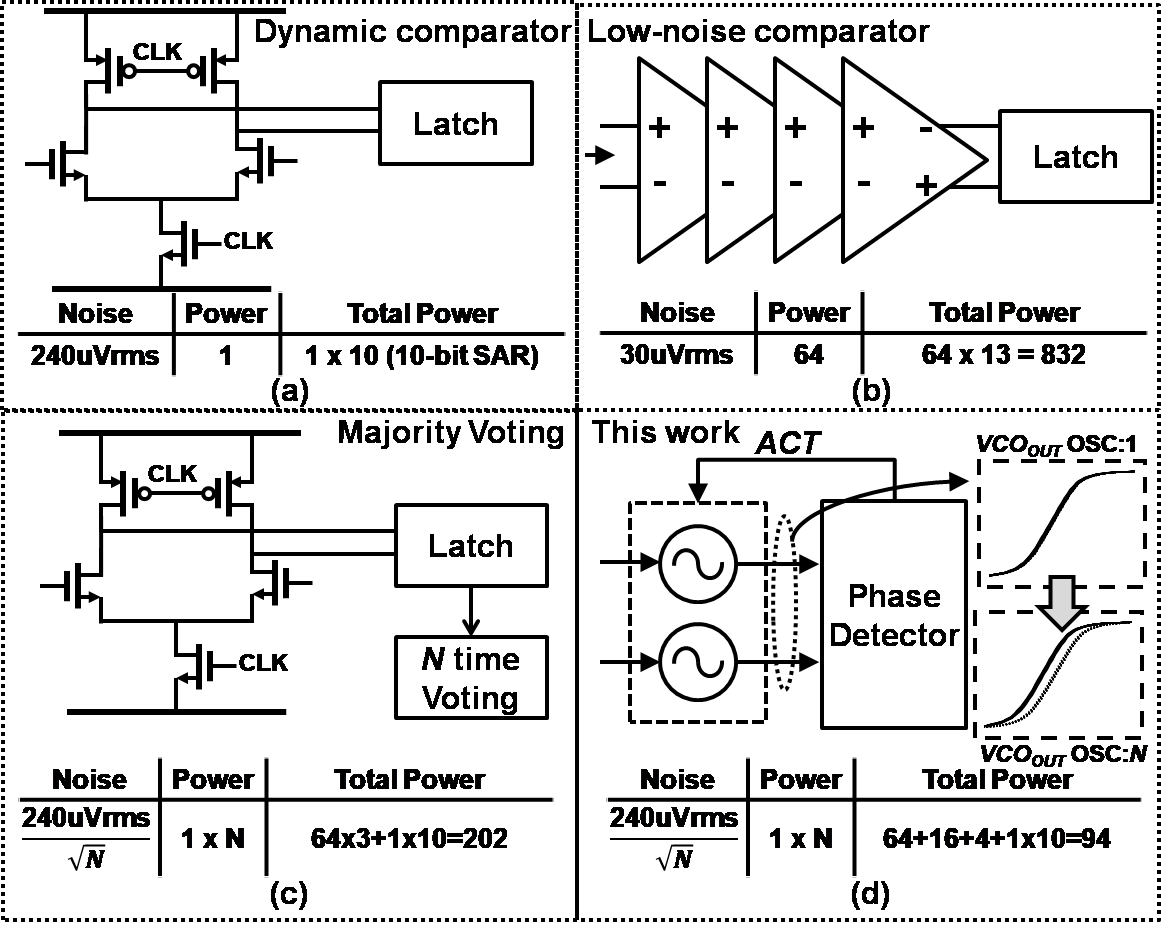
\includegraphics[width=0.5\textwidth]{figs/fig1.png}
  \caption{Comparison of concepts of conventional and proposed low-power comparator designs.}
  \label{fig1}
\end{figure}

We propose a VCO-based comparator that can fully adapt its noise performance depending on the input voltage difference ($\Delta V_{in}$), which minimizes the power consumption of high-precision comparators\cite{yoshioka201413b}. $\Delta V_{in}$ is integrated as a time difference via the VCO, where the integration continues as long as the time difference is below a certain threshold, defined by the phase detector deadzone. For large $\Delta V_{in}$, the oscillation is terminated within a single cycle, and on the other hand, with small $\Delta V_{in}$, the oscillation continues until the integrated time difference exceeds the threshold. The required oscillations to complete the comparison are inversely proportional to $\Delta V_{in}$, realizing a fully adaptive noise and power scaling comparator. This integration opens an "eye" (as in high-speed IO circuits) as the VCO oscillation continues, we name this \textit{eye-opening} technique. 
Compared to the data-driven-noise-reduction (DDNR) comparator\cite{harpe201310b}, which switches between two noise modes based on the comparator's metastable state, the comparator power can ideally be reduced by half.

We demonstrate the concept of the VCO-based comparator with a 13-bit SAR ADC fabricated in 65nm CMOS. The ADC achieves a peak SNDR of 66 dB at 1 MS/s with an FoM of 29 fJ/conv.-step. Since the VCO-based comparator is mainly based on inverters and other simple logic cells, further benefits can be granted by process scaling.
To the best of the author's knowledge, the VCO-based comparator is the first comparator to achieve a fully adaptive noise performance reflecting the input differential levels, and comparators based on eye-opening techniques have been used in a variety of low-power, high-resolution (12-15 bit) SAR ADCs \cite{ding20190, luo2020input, hsieh20180, li2019design, li202065, almarashli2017nyquist, shim2017edge, zhu201914, pan202012, lee2019fast, vogelmann2020efficient}.

This paper expands on ref.\cite{yoshioka201413b} with a detailed analysis of the VCO-based comparator, including its operating principle, noise characteristics, detailed circuit implementation, and noise tolerance under PVT variations.
The paper is organized as follows: Chapter 2 describes the challenges of conventional high-precision comparators, Chapter 3 describes the principle and analysis of the VCO-based comparator, Chapter 4 describes the circuit implementation, and finally, Chapter 5 presents the measurement results and concludes with a summary.

%\section{Comparison of systematic comparator power consumption}
\section{Conventional low-power low-noise comparators}


\begin{figure}[!]
\centering
 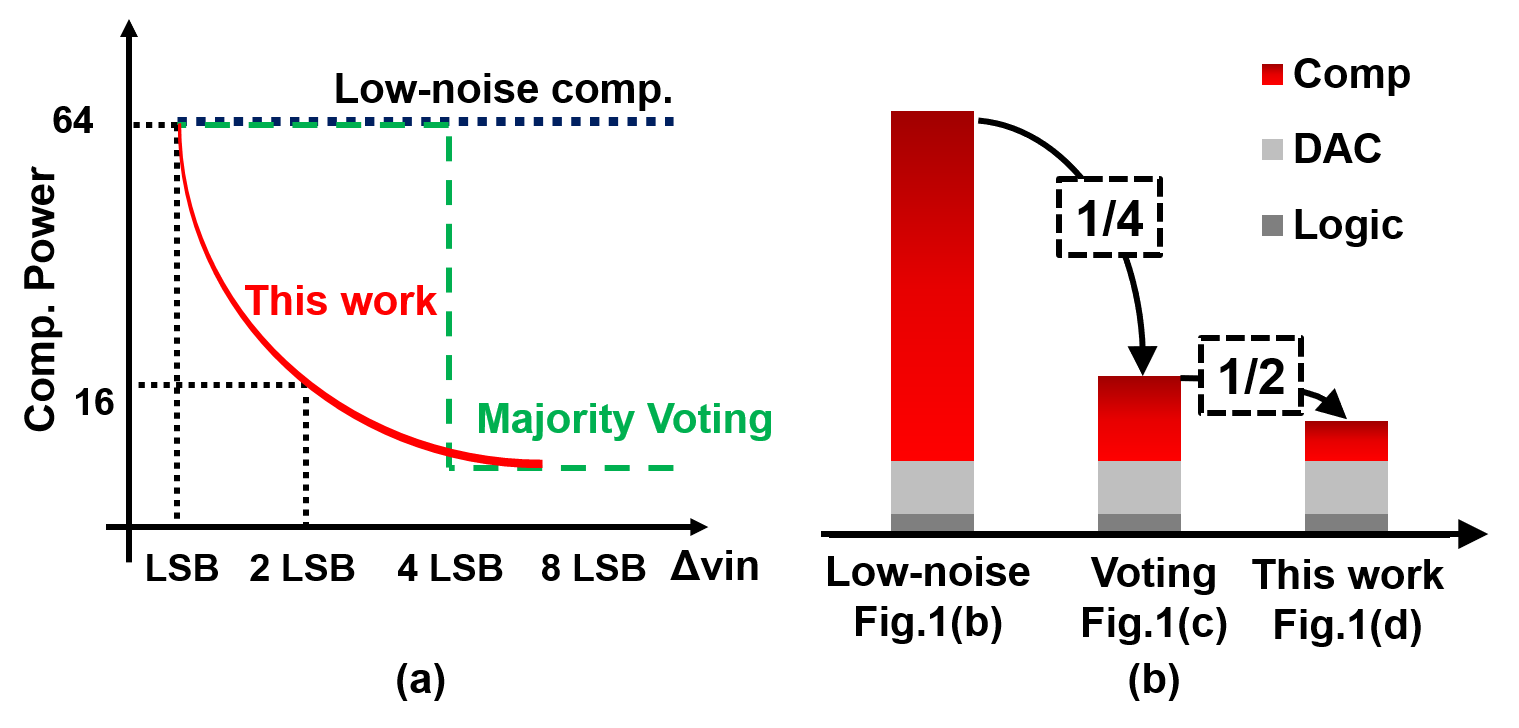
\includegraphics[width=0.5\textwidth]{figs/fig2.png}
  \caption{(a) $\Delta V_{in}$ waveform example during SA conversion.
  (b) $\Delta V_{in}$ versus comparator power consumption.
(c) Improvement in comparator power consumption.
}
  \label{fig2}
\end{figure}
\begin{figure}[!]
\centering
 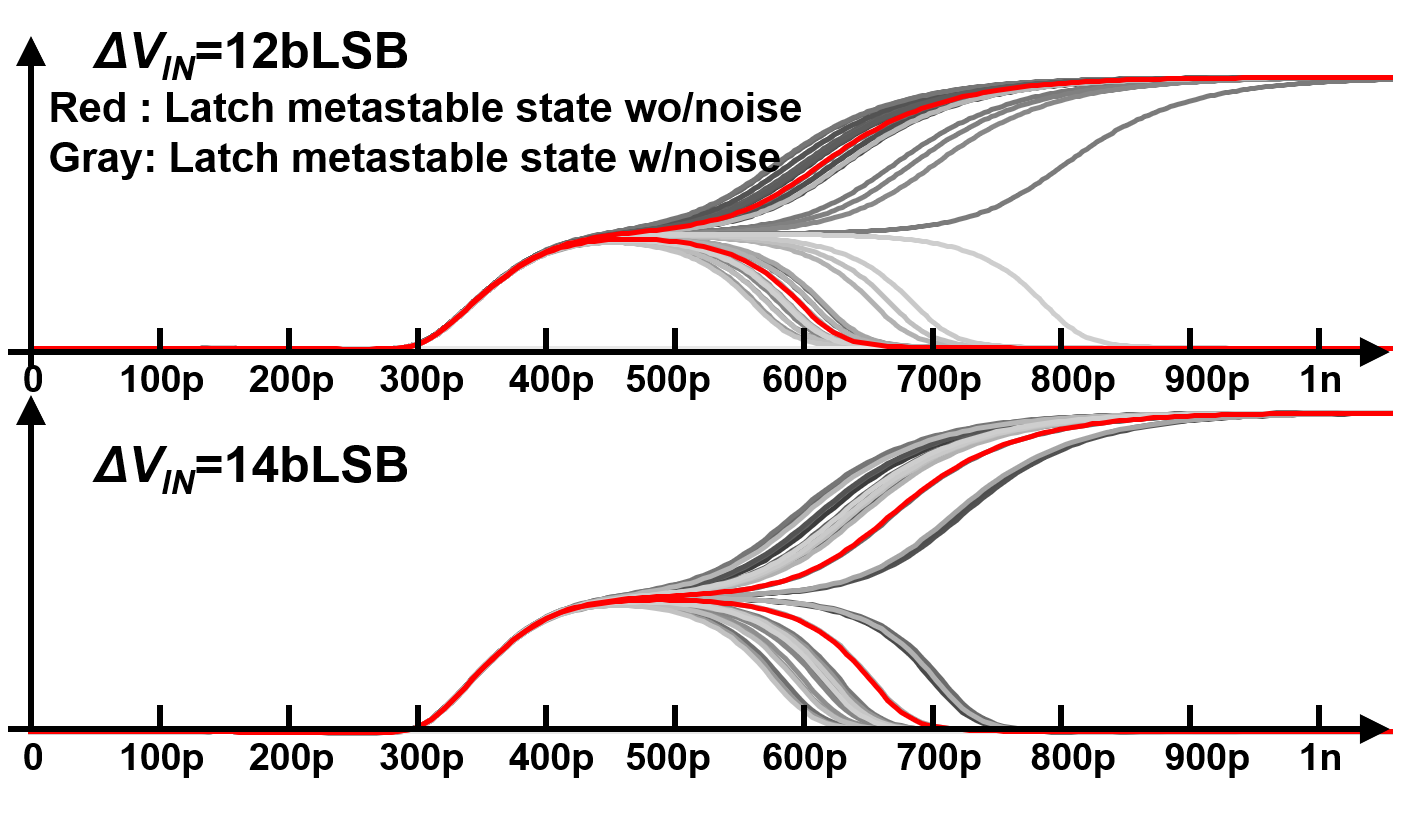
\includegraphics[width=0.4\textwidth]{figs/conventional-strongarm.png}
  \caption{2-stage comparator's latch response when $\Delta V_{in}$ of 2 LSB and 0.5 LSB are given.}
  \label{meta}
\end{figure}

Fig.\ref{fig1}(a) shows a typical comparator used in low-power SAR ADCs\cite{miyahara2008low}, where a typical design has an input-referred noise (IRN) around 10-bit resolution. Fig.\ref{fig1}(b) shows a comparator used in 14-bit SAR ADC \cite{hesener200714b}, the comparator IRN is reduced by cascading preamp stages before the latch. However, as in Fig.\ref{fig2}(a), during the successive approximation (SA) conversion $\Delta V_{in}$ differs each cycle and $\Delta V_{in}<$LSB only occurs once, which is when the comparator noise impacts the bit decision. The comparator noise requirement is relaxed at other cycles and utilizing a low-noise comparator for all of the cycles is inefficient. 

To cut down the comparator power, ref.\cite{harpe201310b} propose a data-driven noise reduction (DDNR) technique, where the comparator triggers majority voting only when the $\Delta V_{in}$ is sufficiently small by monitoring the comparator metastability \cite{shikata20120}. Since the comparator output is decided given the result of $N$ time majority voting, and comparator IRN improves as:
\begin{eqnarray}
    \centering
    V_{voting} = \frac{V_{noise}}{\sqrt{N}}
    \label{voting}
\end{eqnarray}
By switching to a low-noise comparator only when the $\Delta V_{in}$ is small, the total comparator power can be greatly reduced.
Ideally, to halve the comparator IRN, 4x much power must be consumed. Therefore, when the power of the 10-bit resolution comparator is normalized as 1, the power of the 13-bit comparator can be described as:
\begin{eqnarray}
    \centering
    P_{13bcomp} = 1 \times 4^{13-10} = 64
    \label{13b}
\end{eqnarray}
Then, the total comparator power of 13-bit SAR ADC without any power reduction techniques will be:
\begin{eqnarray}
    \centering
    P_{total(Fig.1(b)} = 64 \times 13 = 832
    \label{sar13b}
\end{eqnarray}
Next, we will assume an ideal DDNR done by a 10-bit comparator, where majority voting is triggered when $\Delta V_{in}$ is smaller than 4 LSB (corresponding to 11-bit resolution).
\begin{eqnarray}
    \centering
    P_{total(Fig.1(c)} = 64 \times 3 + 1 \times 10 = 202
    \label{ddnr}
\end{eqnarray}
The analysis shows that comparator power can be reduced by over 1/4 with DDNR. $\Delta V_{in}$ versus comparator power is shown in Fig.\ref{fig2}(b), where the power of the majority voting is plotted in the dashed green line. 
Since the DDNR comparator can only switch between two noise states, the power consumption jumps up when $\Delta V_{in}$ falls below 4 LSB. 
However, for $\Delta V_{in}$ = 4 LSB, the required comparator noise performance is relaxed and is inefficient to use a comparator with a noise performance of 1 LSB.
Thus, the comparison energy can be further reduced if the comparator noise performance can be finely switched reflecting $\Delta V_{in}$ "on-demand".

If the comparator can sense the $\Delta V_{in}$ from its metastable time, on-demand noise control can be achieved by adaptively configuring the number of voting counts.
However, the metastable time of the voltage domain comparator does not directly correlate with $\Delta V_{in}$, making such implementation difficult. For reference, Fig.\ref{meta} shows the 2-stage comparator's latch response when $\Delta V_{in}$ of 2 LSB and 0.5 LSB are given. Without any noise, the regeneration time is inversely proportional to $\Delta V_{in}$ as shown in red. On the other hand, when noise is present, the latch often opens early due to noise effects; $\Delta V_{in}$ cannot be estimated directly from the regeneration time.

We propose a VCO-based comparator that can fully adapt its noise performance reflecting the $\Delta V_{in}$ condition. Thus, the ideal VCO-based comparator's power will depend on $\Delta V_{in}$, as shown in Fig.\ref{fig2}(b). The systematic VCO-based comparator power consumption in this case can be calculated as:
\begin{eqnarray}
    \centering
    P_{total(Fig.1(d))} = 64+16+4+1\times 10=94
    \label{ddnr}
\end{eqnarray}
which is half of that of the DDNR with majority voting (Fig.\ref{fig2}(c)). 
The specific operating principle of the VCO-based comparator is described in the next chapter.

%またTime domain comparators such as delay comparator \cite{agnes20089} はプロセススケーラビリティと低電力動作能力を持ち、発展が期待されている. 一方でこれらのnoise characteristics are not enough for high-resolution ADCs.

\begin{figure*}[!]
\centering
 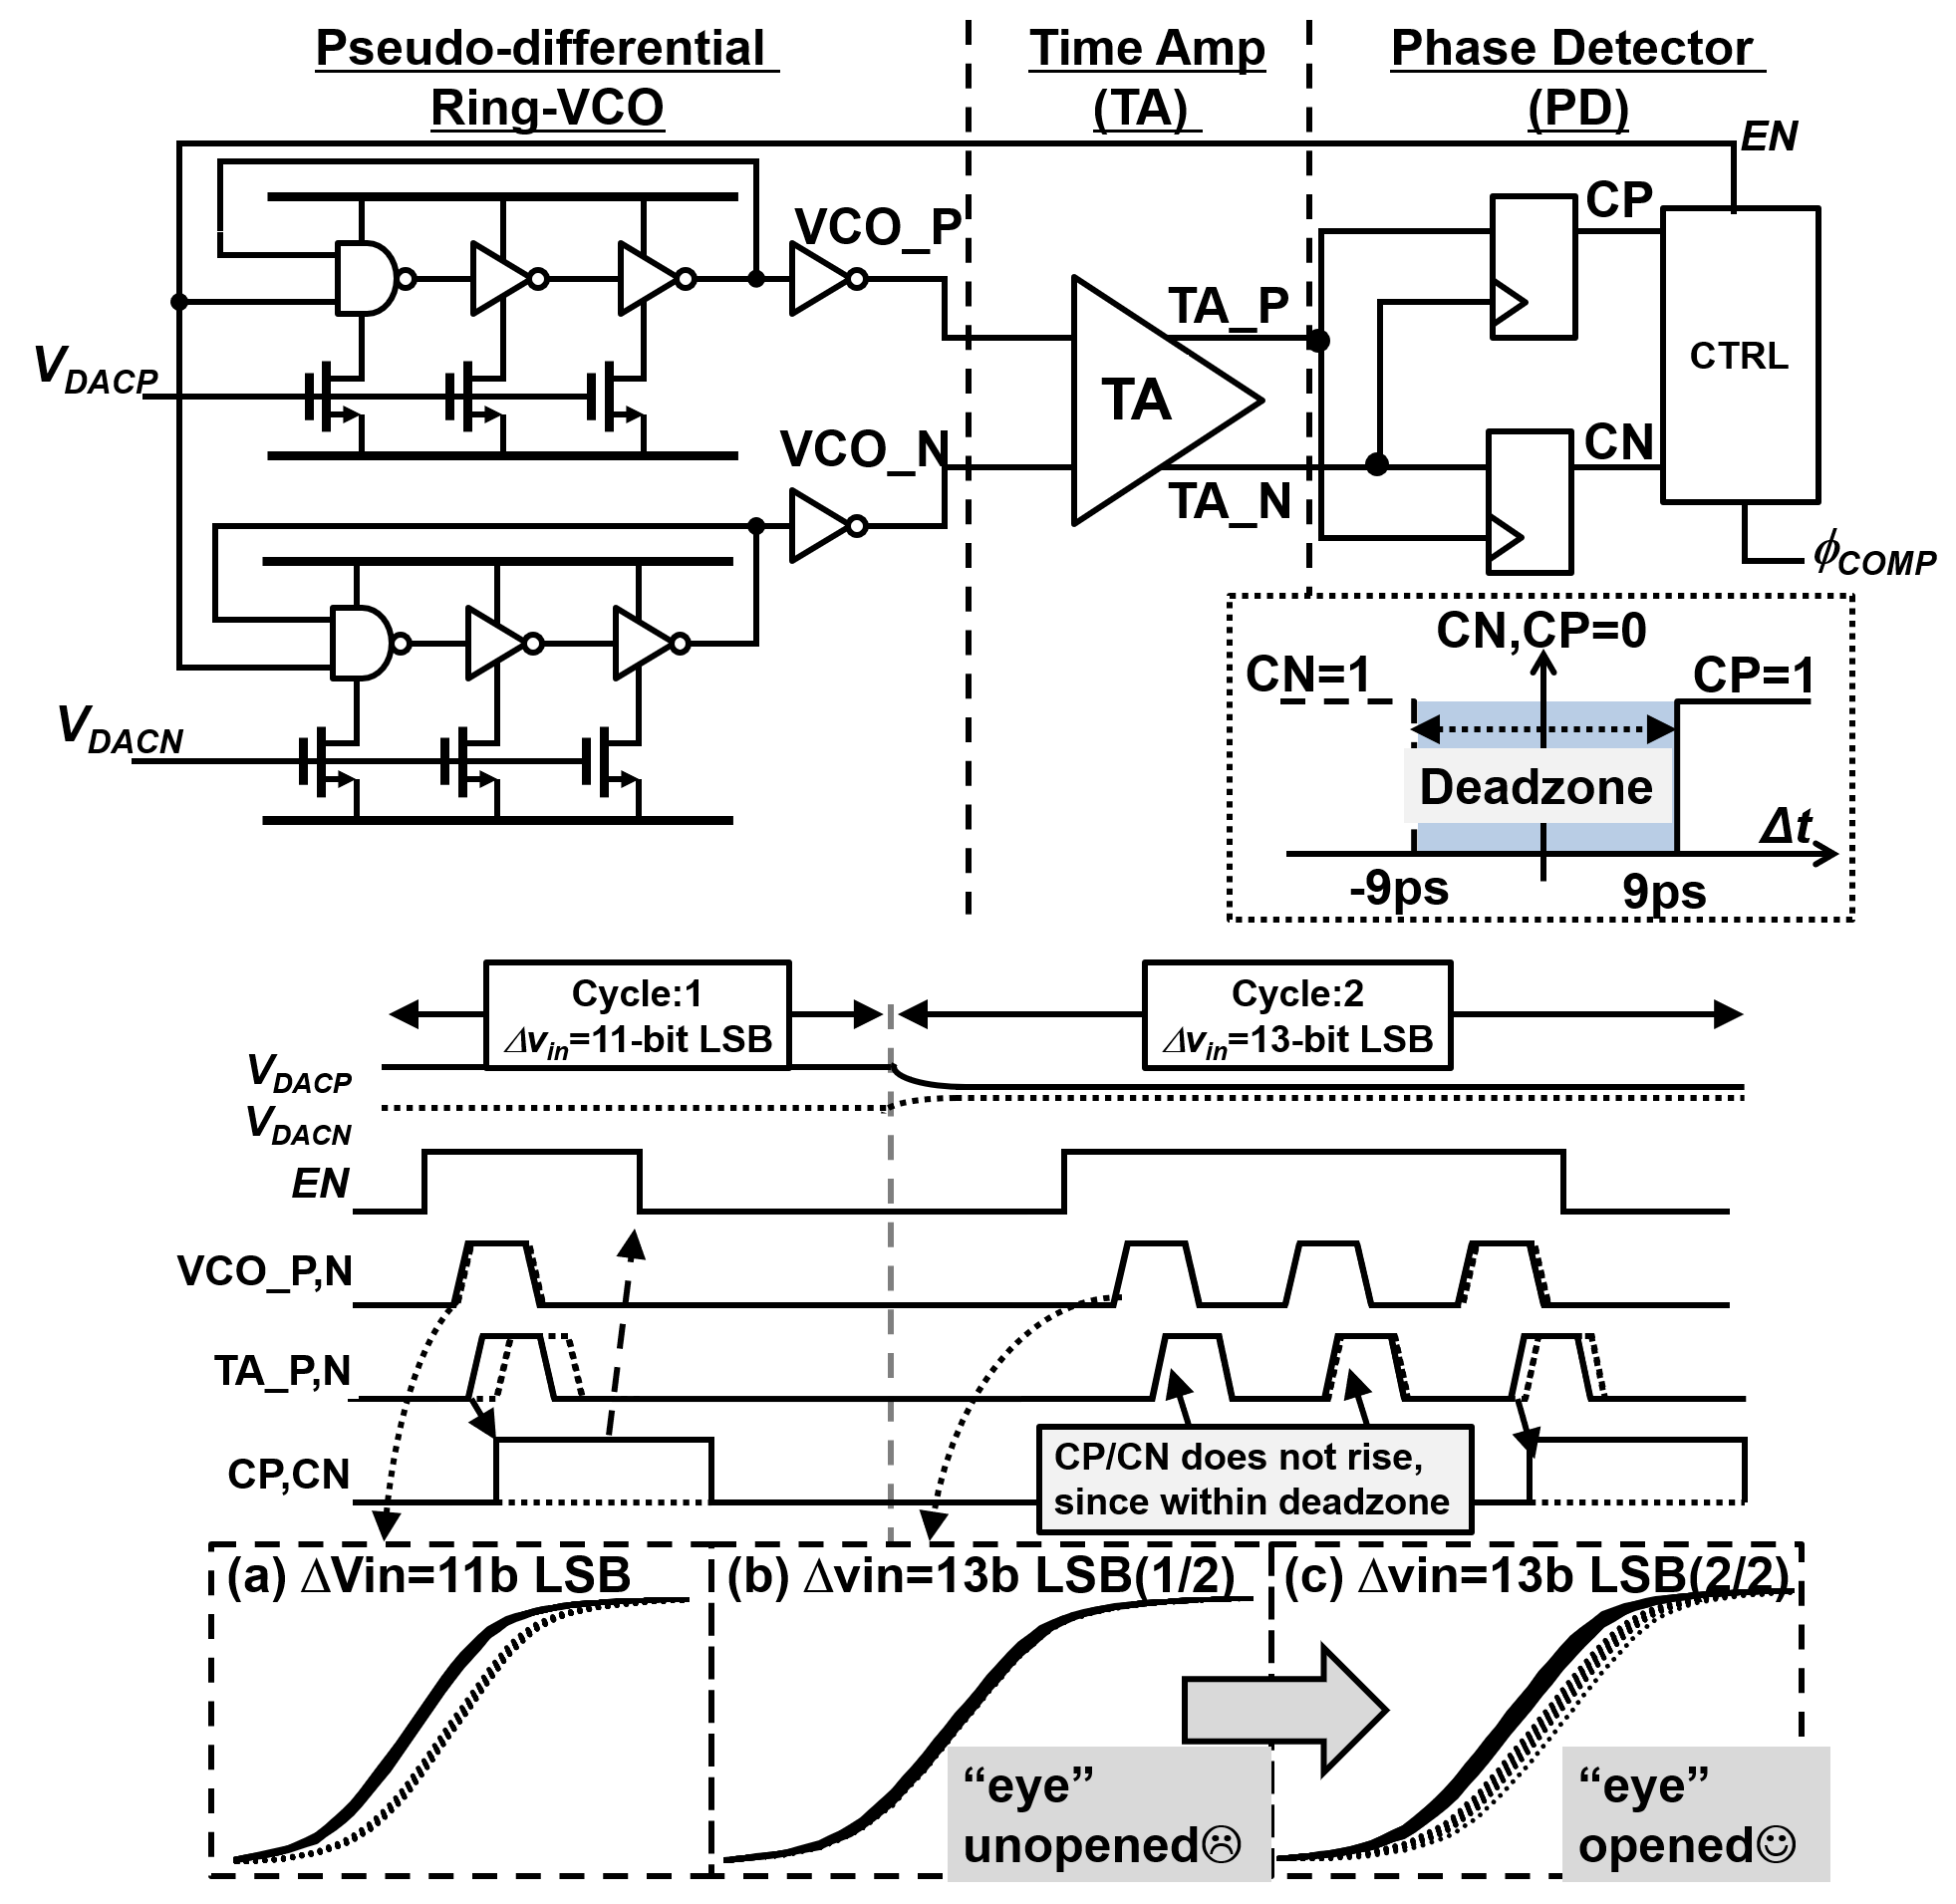
\includegraphics[width=0.9\textwidth]{figs/fig4.png}
  \caption{VCO comparator block diagram and its timing chart. (a)-(c) shows the VCO waveform when $\Delta V_{in}$=11-bit LSB and 13-bit LSB are given, respectively.}
  \label{schema}
\end{figure*}

\section{VCO-based comparator}
\subsection{VCO-based comparator fundamentals}
Fig.\ref{schema} shows the conceptional schematic of the VCO-based comparator. Similar to delay line-based comparators\cite{agnes20089}, the C-DAC analog voltages($V_{DACP}$, $V_{DACN}$) are given to control the oscillating frequency of the ring oscillator. We utilize a time amplifier (TA)\cite{lee20089} to amplify the time difference between the VCO outputs ($VCO_P$, $VCO_N$). Finally, the TA outputs ($TA_P$, $TA_N$) are connected to the phase detector (PD), which resolves the comparison results.

The lower part of Fig.\ref{schema} shows the VCO-based comparator operation in the case of large and small $\Delta V_{in}$, respectively. In this example, at cycle 1, $\Delta V_{in}$ is fairly large ($>$11-bit LSB) where the VCO-based comparator adaptively operates as a delay line-based comparator. When $EN$ rises, the VCOs are "enabled" and pulses start to travel through the ring-VCO inverter cells. The pulses reach the TA and their time difference is amplified. In this case, $TA_P$ rises faster than $TA_N$ with sufficient margins and the D-FF-based phase detector resolves the comparison results: CP=1 and CN=0. Once the comparison results are obtained, $EN$ is set down to “disable” the ring-VCO, which resets the ring-VCO phase state and prevents unnecessary oscillations.

Next, the comparator operation with small $\Delta V_{in}$ (Cycle 2 in Fig.\ref{schema}) is explained. Similarly, $EN$ rise and the pulses transmit through the VCOs. Fig.\ref{schema}(a) and (b) plot the VCO outputs of 50-times transient noise simulation with $\Delta V_{in}$ of 4 and 1 LSB, respectively. Note that in (b), an “eye” is not opened because the VCO jitter is larger than the input-dependent time difference. In such conditions, the comparator cannot make correct decisions and noise reduction is required.

In VCO-based comparators, the event of small $\Delta V_{in}$ is detected by exploiting the deadzone property of the D-FF based PD. It is known that D-FFs require a finite setup and hold time to produce an output: if the input time difference between the data and the clock is too short ($<$9ps in 65nm CMOS), a "deadzone" occur where the output does not respond.
As in cycle 2 of Fig.\ref{schema}, when the $TA_P$ and $TA_N$ difference is small and within the deadzone, the VCO automatically continues the oscillation (or signal integration) until the time difference is large enough to exceed the deadzone. \textcolor{red}{In Fig.\ref{schema}(c), the TA output exceeds the deadzone after 3 oscillations and “eye-opening” is observed. Such utilization of VCOs and the deadzone allows adaptive configuration of the comparator noise reflecting the $\Delta V_{in}$ level.}


\begin{figure}[!]
\centering
 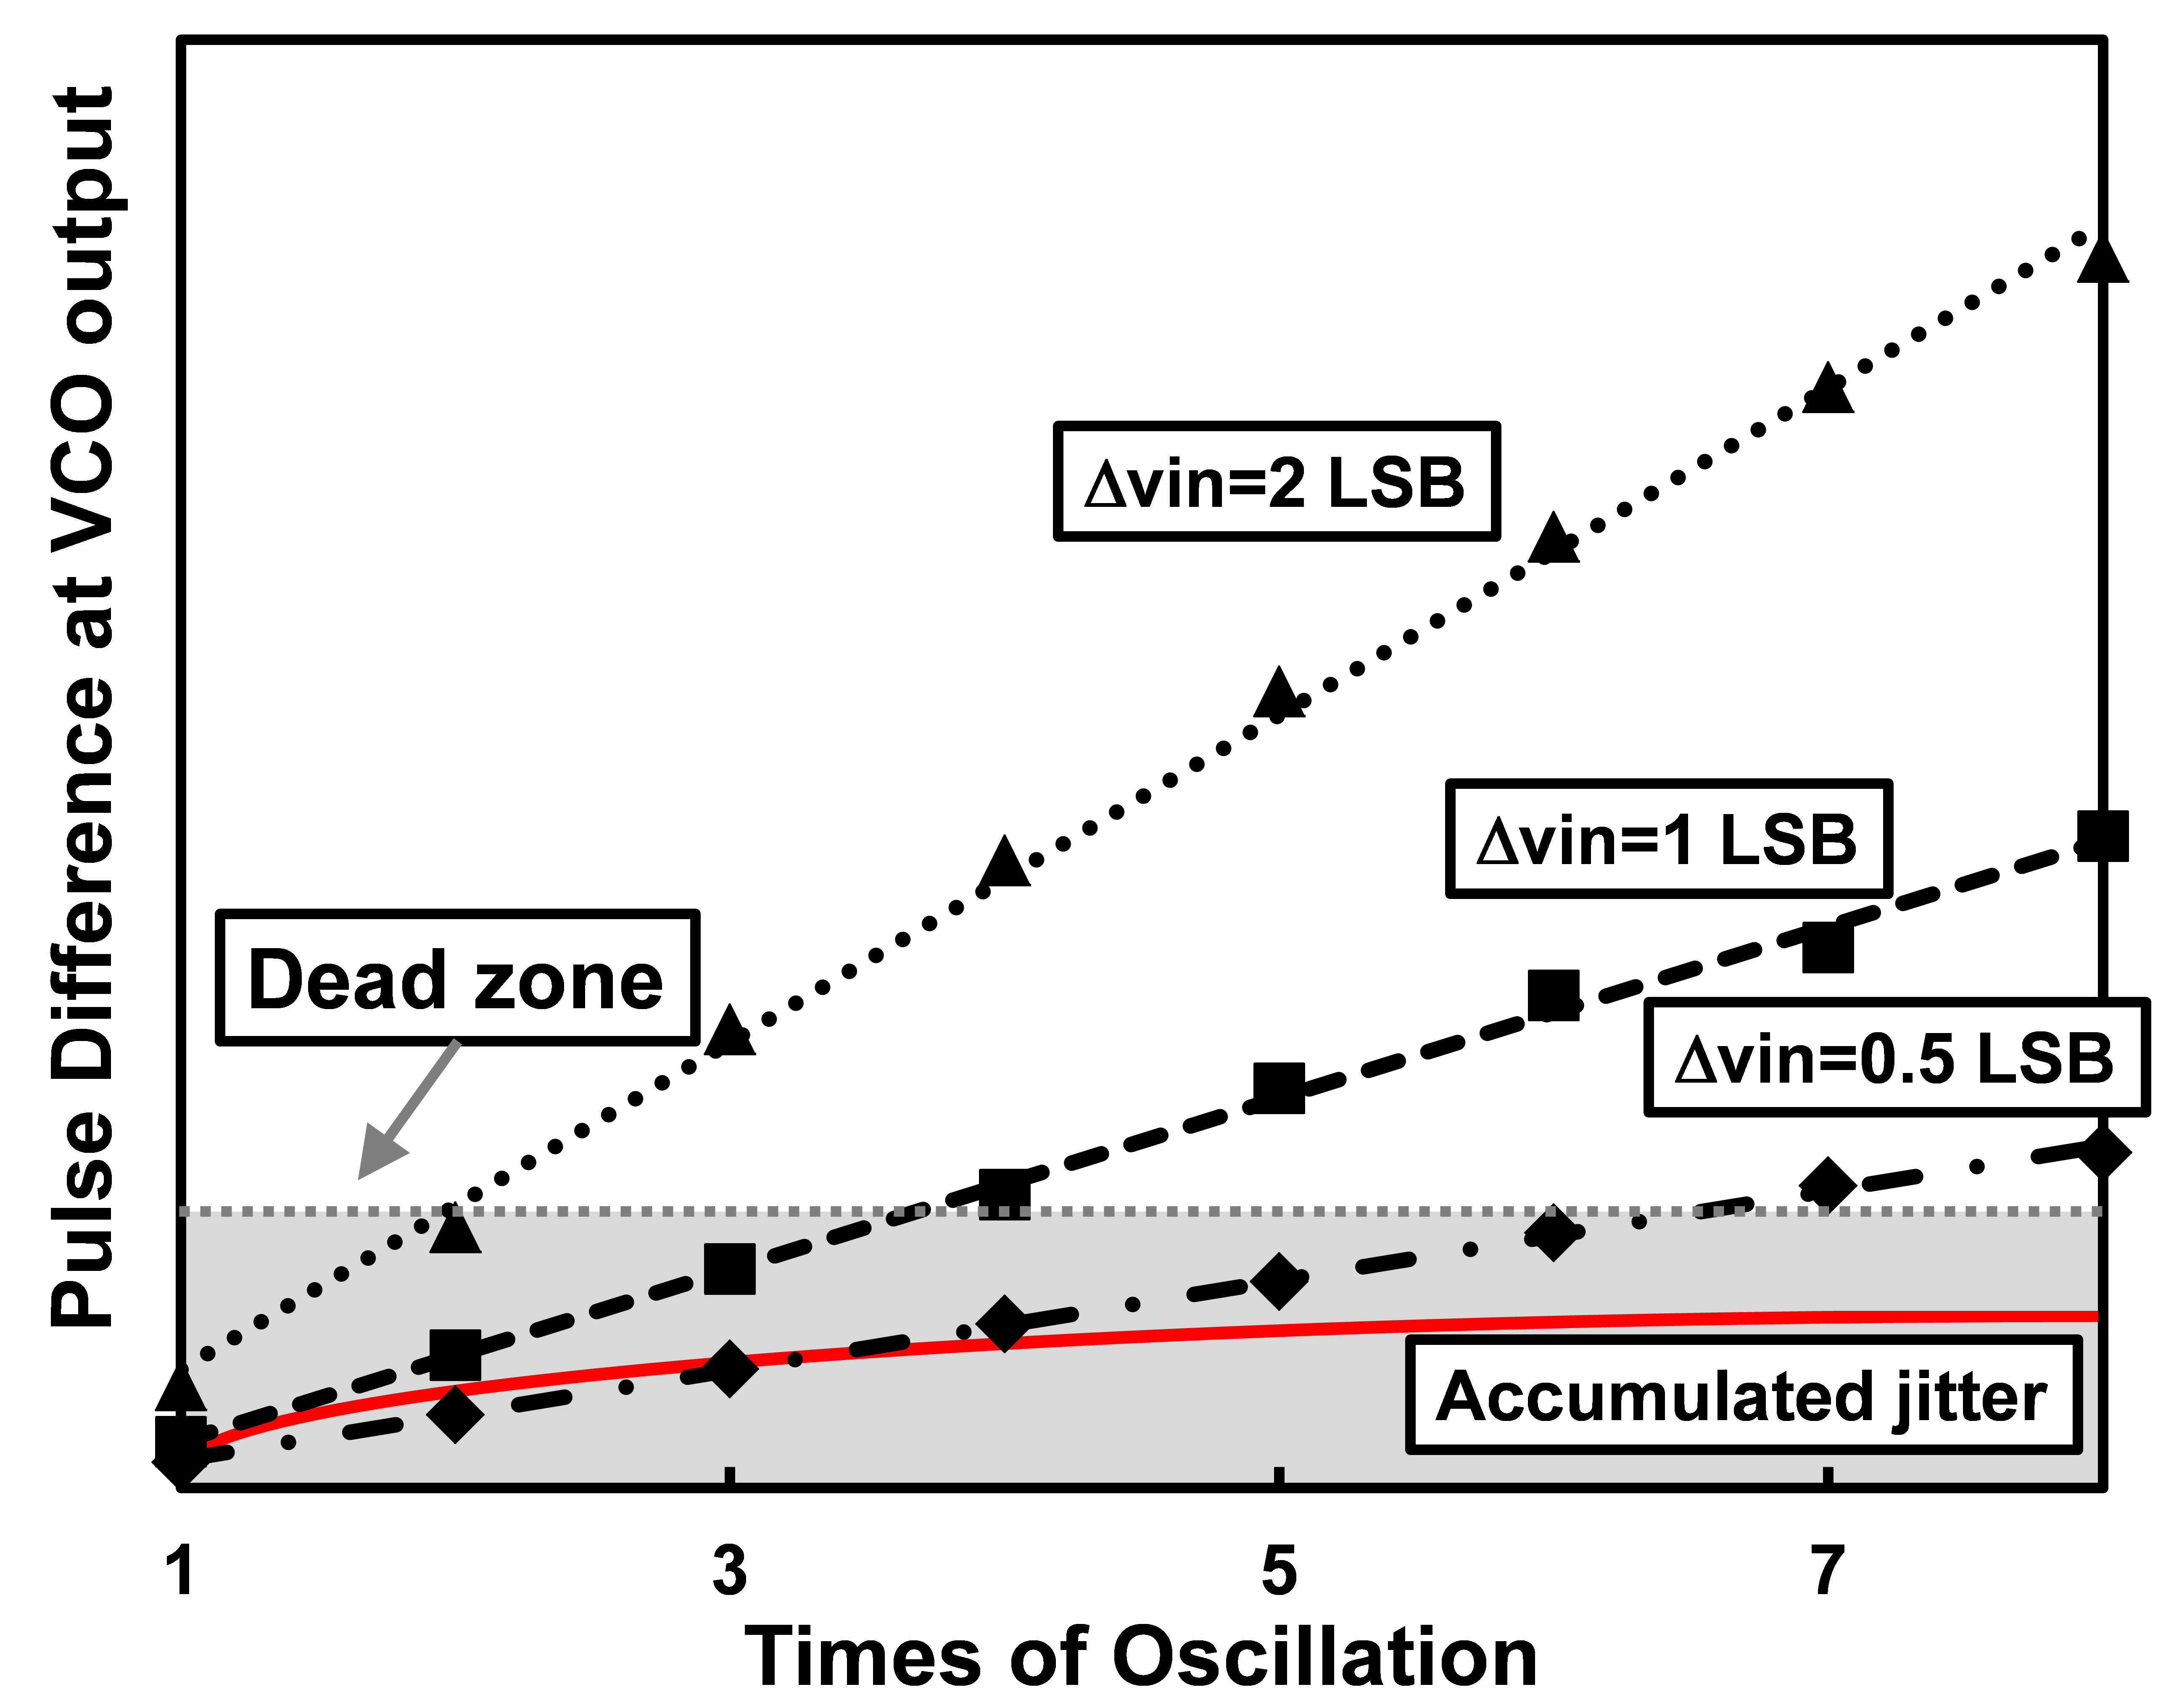
\includegraphics[width=0.5\textwidth]{figs/fig5.png}
  \caption{Principle of the eye-opening operation is shown, where the signal-dependent time difference outperforms the accumulated jitter as the oscillation continues.}
  \label{fig5}
\end{figure}

An initial study of the VCO-based comparator's noise reduction is explained with the aid of Fig.\ref{fig5}, where the simulation result of the Number of Oscillations ($N$) vs VCO pulse difference is shown. % for $\Delta V_{in}$ of 11-bit, 12-bit, and 13-bit LSB, respectively. 
We can observe that $N$ and pulse differences have a linear relationship of $\alpha \Delta V_{in}N$, where $\alpha$ is the VCO voltage-time conversion gain. On the other hand, the VCO accumulated jitter is proportional to $\sqrt N$\cite{hajimiri1999jitter,abidi2006phase}. In the case of $\Delta V_{in}$ = 13-bit LSB, even though the jitter may be dominant at 1-3 times of oscillation, the signal-dependent pulse difference will overcome the jitter as $N$ increase. The area in gray indicates the deadzone: as long as the pulse difference is within the deadzone, the oscillation will continue. The detailed VCO-based comparator's noise design guide is given in the next section.
%Therefore, by careful design of the deadzone and VCO jitter, we can design VCO-based comparators with the desired noise performance.

\subsection{Noise design guideline of VCO-based comparators}
The most important aspect of designing a high-precision comparator is the noise design; this section discusses the noise design guidelines for VCO-based comparators. Although the noise analysis of VCO-based comparators is described in detail in ref.\cite{luo2020input, ding20190}, the comparator design guidelines are not discussed. %(どういうこと?) 
Designing a VCO-based comparator satisfying a desired noise involves two major steps:
\begin{itemize}
\item Firstly, the VCO block is designed as a delay line-based comparator which satisfies a certain noise. %Since accurate comparison can be achieved by eye-opening operation, as a rule-of-a-thumb, the noise of the delay line based comparator should be around $4\times$ worse than the target IRN to obtain sufficient power savings.
\item To obtain the peak noise performance, the VCO-referred deadzone is set by configuring the TA gain.
\end{itemize}

The first step is to design the VCO block as a delay line-based comparator satisfying a certain noise.
Following ref.\cite{timecomp}, the jitter of a unit delay stage can be calculated as:
\begin{eqnarray}
    \centering
    jitter_{unit} = \frac{\sqrt{C_L\beta k \rm{T}}}{I_{DS}}
    \label{jit}
\end{eqnarray}
where $\beta$ is the product of $g_m$, $r_o$, and noise factor $\gamma$ and $I_{DS}$ is the inverter current when $V_{in} = V_{DD}/2$ and $k$ is Boltzmann’s constant.
The unit stage's voltage-time conversion gain can be obtained with the analysis in ref.\cite{timecomp} as: 
\begin{eqnarray}
    \centering
    \rm{Gain} = \frac{g_mC_LV_{DD}}{2I_{DS}^2}
    \label{gain}
\end{eqnarray}
From eq.(\ref{jit}) and (\ref{gain}), the $N_{inv}$ stage delay line-based comparator $IRN_{DL}$ with NMOS voltage-time conversion can be derived as:
\begin{eqnarray}
    \centering
    IRN_{DL} = \frac{\sqrt{jitter}}{\rm{Gain}} = \frac{1}{\sqrt{N_{inv}C_L}}\frac{2I_{DS}\sqrt{2\beta k\rm{T}}}{V_{DD}g_m}
    \label{delaylineIRN}
\end{eqnarray}

\begin{figure}[!t]
\centering
 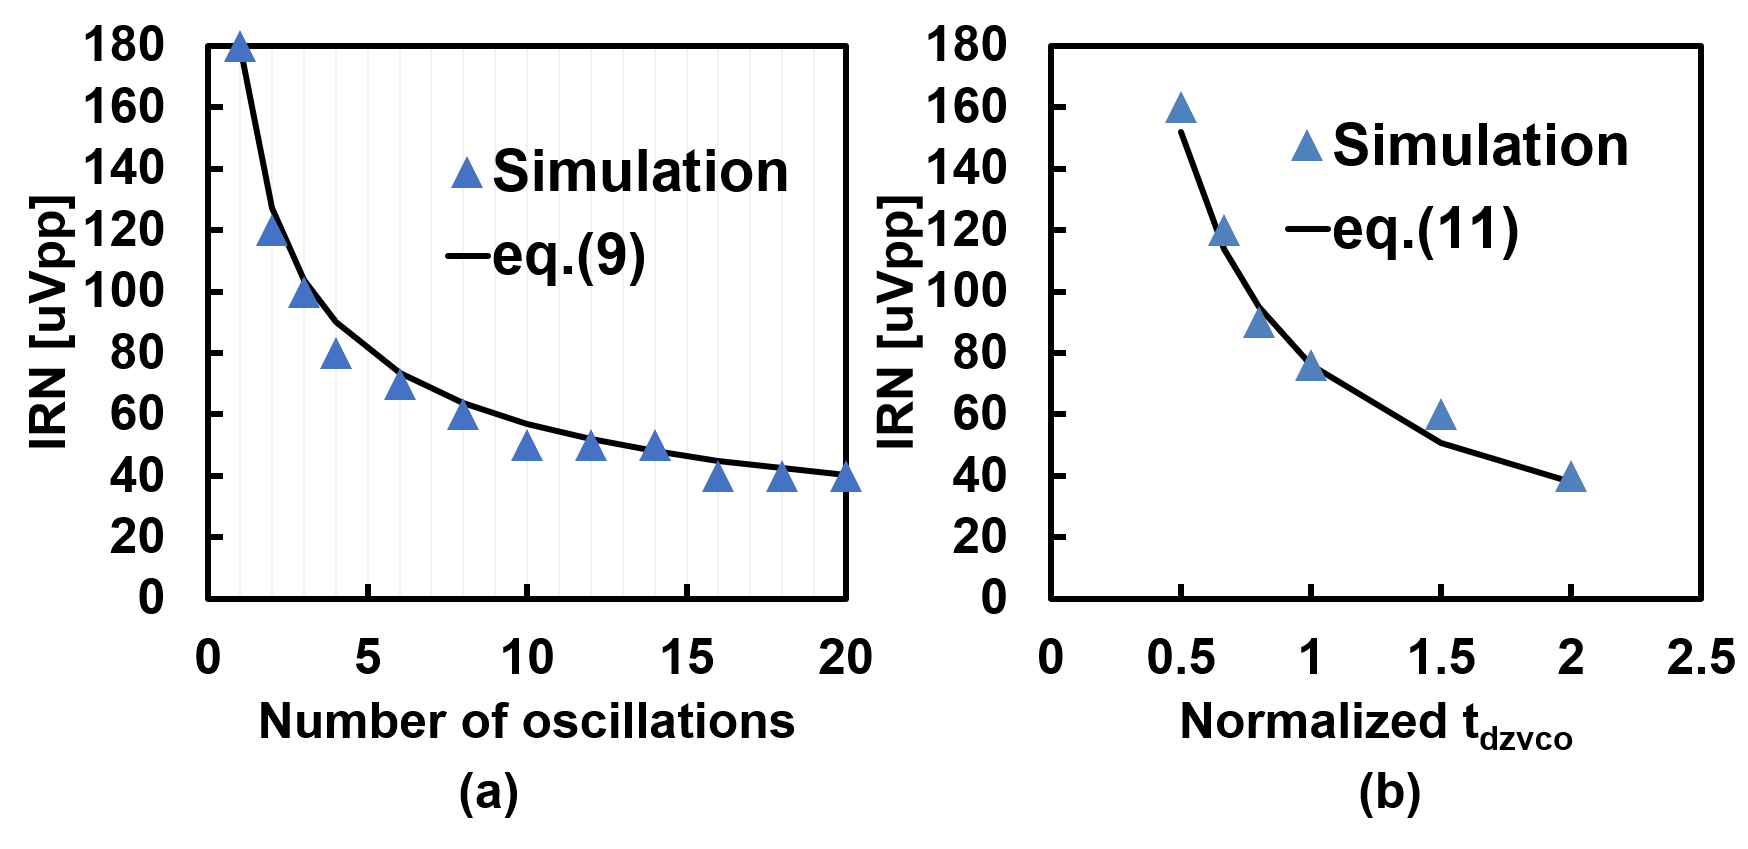
\includegraphics[width=0.5\textwidth]{figs/analysis.png}
  \caption{(a) Number of oscillations versus $IRN_{VCO}$ is shown, comparing eq.(9) and noise simulation results. (b) $t_{dzVCO}$ versus $IRN_{VCO}$ is shown, comparing eq.(11) and noise simulation results.}
  \label{nocnoise}
\end{figure}

As discussed in Fig.\ref{fig5}, the VCO-based comparator integrates the signal by oscillation to improve $IRN_{VCO}$.
The relationship between the number of oscillations $N$ and $IRN_{VCO}$ is as follows.
\begin{eqnarray}
    \centering
    IRN_{VCO} = \frac{IRN_{DL}}{\sqrt{N}}
    \label{vcoIRN}
\end{eqnarray}
Fig.\ref{nocnoise}(a) confirms that eq.(\ref{vcoIRN}) holds in transient noise simulation. Note that the state at the $N$ = 1 is equivalent to $IRN_{DL}$.

%ちゃんとした解析を足す
%Due to the adaptive noise performance characteristics of the VCO-based comparator, the noise requirements of the $IRN_{DL}$ itself are relaxed. As a rule of thumb, to minimize the overall comparator power, the target $IRN_{DL}$ should be about four times worse than the peak IRN to achieve a good balance between the VCO-based comparator power consumption and noise. %For example, we can try to maximize the input transistor $g_m$ in eq.(\ref{delaylineIR}).

% deadzoneの効果。VCOからみたdeadzoneはDFF deadzone/TA gain。
Next, we show that VCO-based comparator noise can be configured by tuning the VCO-referred deadzone.
First of all, due to the time amplifier, the deadzone seen from the VCO output ($t_{dzvco}$) is compressed by the TA gain $G_{TA}$.
\begin{eqnarray}
    \centering
    t_{dzvco} = \frac{t_{dz}}{G_{TA}}
    \label{dzvco}
\end{eqnarray}
Importantly, $IRN_{VCO}$ is inversely proportional to the deadzone, as analyzed in ref.\cite{luo2020input, ding20190}. Thus, from eq.(\ref{dzvco}), we can derive:
\begin{eqnarray}
    \centering
    IRN_{VCO} \propto \frac{IRN_{DL}}{t_{dzvco}} = \frac{IRN_{DL}\times G_{TA}}{t_{dz}}
    \label{irn}
\end{eqnarray}
Interestingly, this shows that by tuning $G_{TA}$, we can directly tune the VCO-based comparator IRN. Note that directly tuning $T_{dz}$ is difficult, and tuning $IRN_{DL}$ has a large impact on the comparator power. On the other hand, $G_{TA}$ can be easily tuned by the time amplifier's capacitive load without large power overheads and provides great flexibility in the comparator noise design. To confirm eq.(\ref{irn}), we used transient noise simulation and swept $t_{dzvco}$ by configuring the $G_{TA}$ and measured $IRN_{VCO}$ (Fig.\ref{nocnoise}(b)) and simulations  matches eq.(\ref{irn}) well. We would also like to note that the actual $IRN_{VCO}$ includes the noise from TA and PD as well. In our design, the total noise of TA and PD was about 1/4 of the entire $IRN_{VCO}$, so there is no significant deviation from eq.(\ref{irn}).

\subsection{Power-speed tradeoff analysis}
\begin{figure}[!]
\centering
 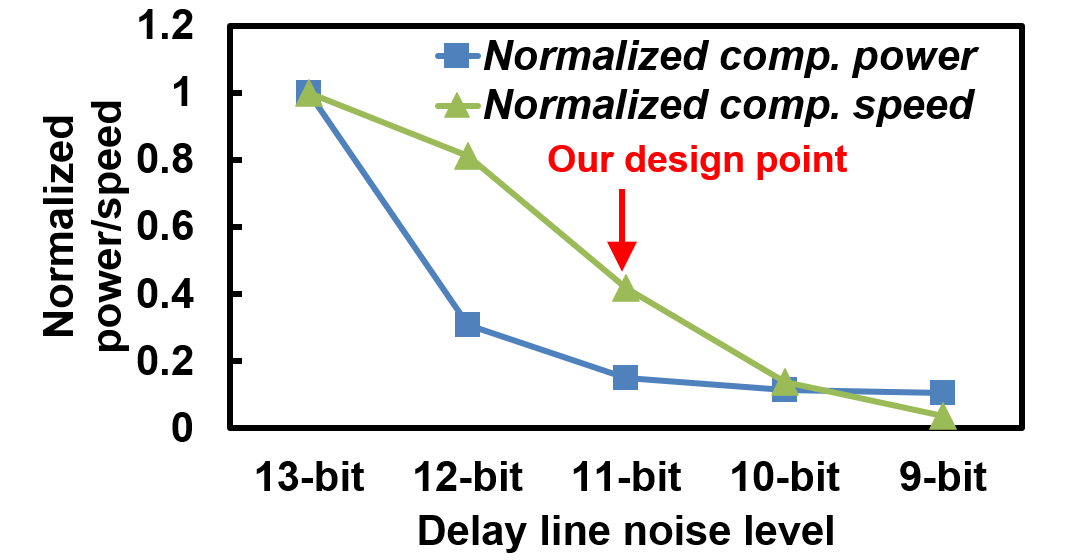
\includegraphics[width=0.5\textwidth]{figs/comp_anal.png}
  \caption{Simulated results for $IRN_{DL}$ versus comparator power and speed, respectively. The VCO-based comparator essentially trades speed for power, and $IRN_{DL}$=11-bit level provides a good balance between speed and power.}
  \label{comp-anal}
\end{figure}
The VCO-based comparator can be viewed as a comparator that essentially trades speed for power.
To analyze this point in-depth, the comparator power and speed when $IRN_{DL}$ is swept are summarized in Fig.\ref{comp-anal}.
Here, to simplify the analysis, the comparator power and speed are calculated from the results of SA operations in a system simulation in which the VCO-based comparator is adapted to a 13-bit SAR ADC.

If $IRN_{DL}$ has a noise performance of 13-bit LSB level, the comparator ideally has almost no oscillation and operates similarly to the low-noise comparator in Fig. 1(b); the speed is excelling but is power-hungry. The power consumption can be greatly reduced by lowering $IRN_{DL}$ to 12-bit and 11-bit and adapting eye-opening operations. On the other hand, the time required for a small $V_{in}$ comparison becomes longer and the comparator speed decreases. The point where $IRN_{DL}$=11-bit LSB has an excellent power-speed trade-off balance and was also adopted in our prototype design: the comparator power can be reduced to 1/8 of that when $IRN_{DL}$=13-bit LSB and the comparator speed is twice as long as the penalty. If $IRN_{DL}$ is further relaxed, the power reduction effect is saturated and the benefit is small. For example, if $IRN_{DL}$=10-bit LSB, the power consumption can be further reduced by 25\%, but the speed will be degraded by a factor of 3.

\subsection{PVT drift resistance}
\begin{figure}[ht!]
\centering
 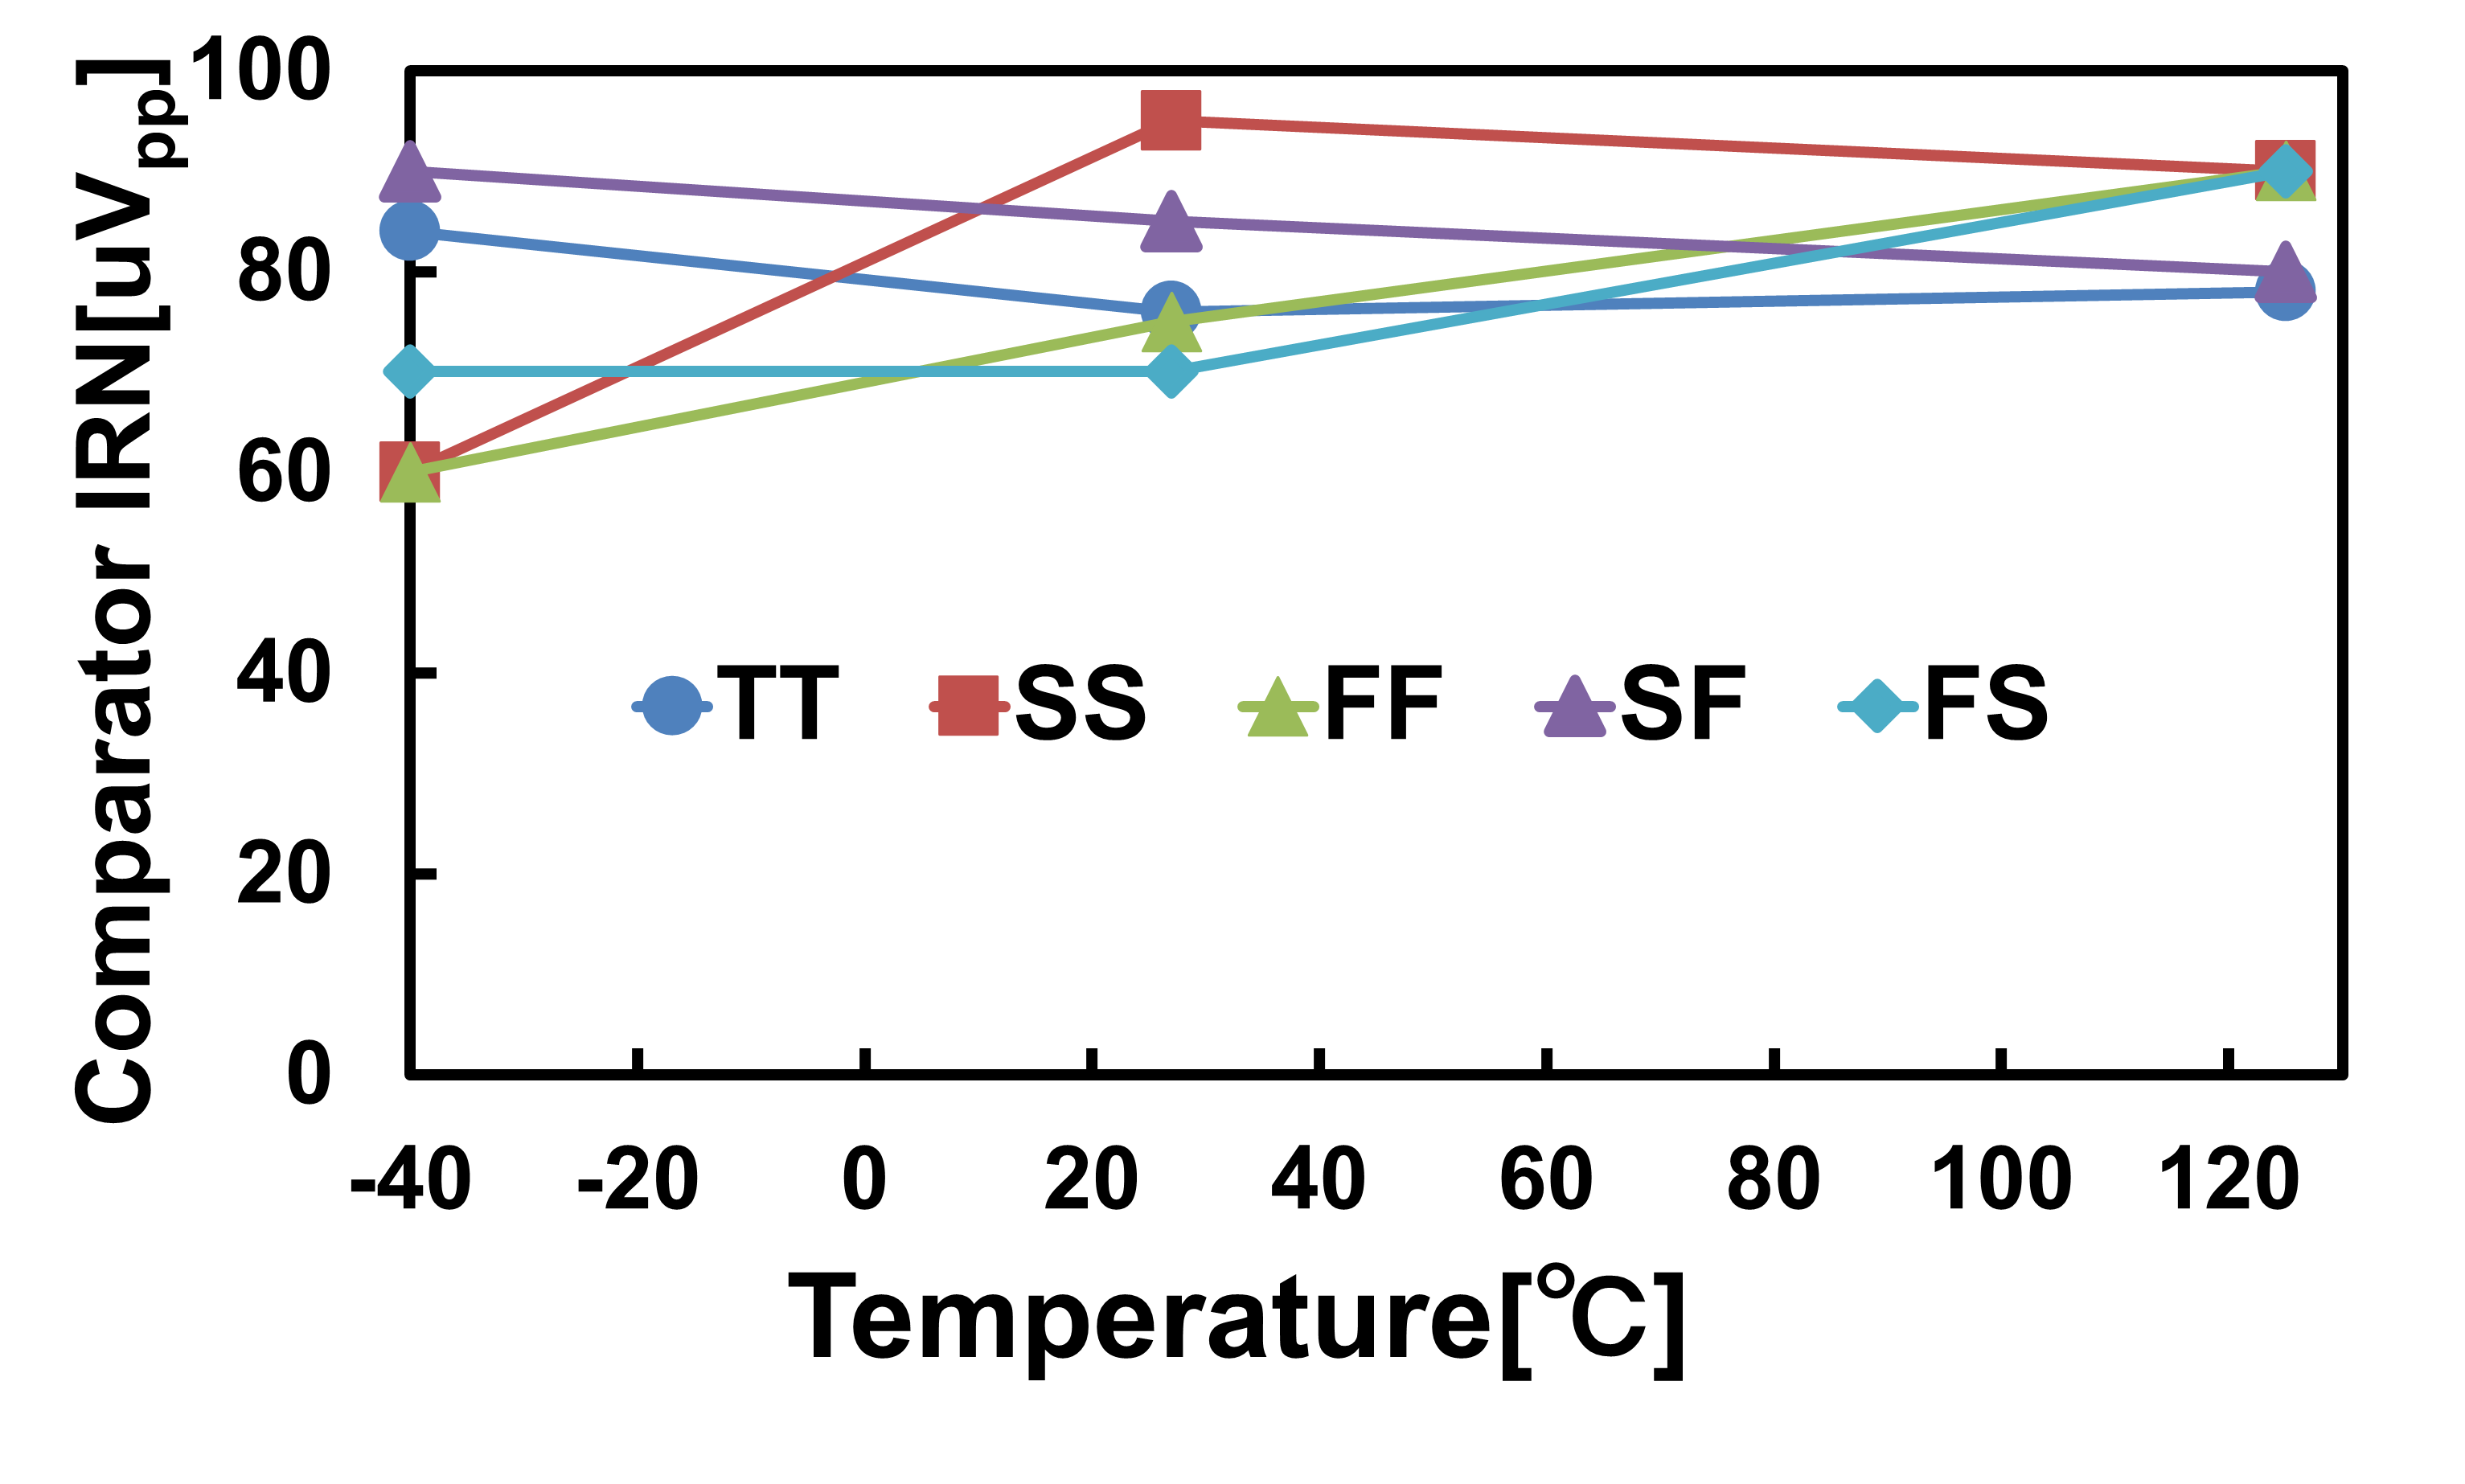
\includegraphics[width=0.5\textwidth]{figs/pvt_vco.png}
  \caption{Simulated $IRN_{VCO}$ characteristics throughout the PVT variation.}
  \label{pvtvco}
\end{figure}

One of the major issues in high-precision comparators is the noise drift due to PVT variations. In general, comparator noise records its worst value at  FF high-temperature corners where current and thermal noise increase and it is necessary to suppress the noise under these conditions. In this section, we show that the VCO-based comparator suppresses the noise drift due to PVT variation by exploiting the PVT vs. $g_m$ dependence of the time amplifier.

Eq. (\ref{delaylineIRN}) shows that at FF high-temperature, $IRN_{DL}$ worsens as in normal comparators.
Interestingly, since $G_{TA}$ is inversely proportional to $g_m$, the time amplification gain becomes smaller under FF high-temperature conditions. Thus, the VCO-referred deadzone becomes smaller, which is a shift that improves the IRN of the VCO-based comparator according to eq.(\ref{irn}). As a result, $IRN_{DL}$ and $G_{TA}$ cancels each other out, and the noise growth at FF conditions can be suppressed. The simulated $IRN_{VCO}$ with PVT variations is shown in Fig.\ref{pvtvco}. Even under the most severe FF high-temperature conditions, the IRN increases only 18\% compared to TT conditions. On the other hand, the noise worsens at SS corners as well, due to the increase in $G_{TA}$. We would like to note that even under this condition, the IRN increase was about 20\% compared to TT conditions.

\begin{figure*}[!]
\centering
 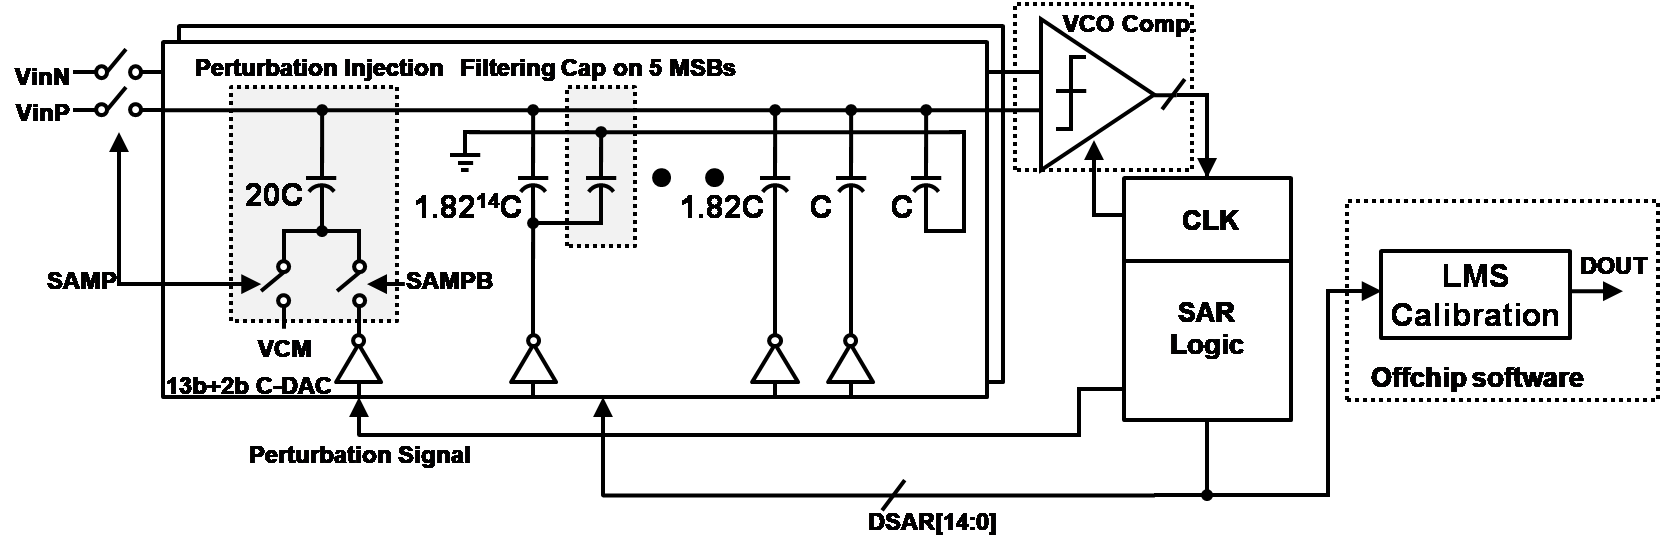
\includegraphics[width=1\textwidth]{figs/fig7.png}
  \caption{Our proof-of-concept 13-bit SAR ADC architecture. The C-DAC non-linearity is calibrated with off-chip software, using perturbation injection\cite{liu201012b}.}
  \label{13bsar}
\end{figure*}

\subsection{Metastability detection}
Since the comparator accuracy is proportional to the metastable time, high-precision comparators have the risk of conversion errors in asynchronous SAR ADCs and thus, metastable detection is necessary.
Conventional comparators often implement metastable detection by directly monitoring the comparison time, but these have a large PVT dependency and require calibration\cite{shikata20120}.

On the other hand, a VCO-based comparator intrinsically has a metastable detecting function which does not require PVT calibration. In the case of metastability, the VCO time difference remains within the deadzone and the VCO continues to oscillate. Therefore, metastable detection can be achieved by simply counting the number of oscillations. In our design, the number of VCO oscillations is monitored by a counter circuit, and when the number of oscillations exceeds 10 times, metastability is detected and a random result is stored. By using this intrinsic metastability detection of VCO-based comparators, we can implement e.g. additional bit judgment \cite{shikata20120, ding20190} and DAC calibration \cite{zhu201914} with less PVT dependency.

\section{Circuit Implementations}

\subsection{13-bit SAR ADC implementation}
To demonstrate the high-accuracy VCO-based comparator, we design a proof-of-concept 13-bit low-power SAR ADC.
The entire 13-bit SAR ADC architecture is shown in Fig.\ref{13bsar}. To cut down the C-DAC power, we utilize a sub-binary C-DAC with perturbation logic for LMS calibration as in ref.\cite{liu201012b}. The C-DAC has 2-bit redundancy implemented with a sub-binary radix of 1.82. To suppress the noise of C-DAC buffers, filtering capacitors\cite{miki20154} are provided until the 5th MSB bit. Unit capacitor (C) of 0.5fF was chosen to meet the kT/C noise requirements.

To cancel the capacitor mismatch effect, perturbation-based digital calibration\cite{liu201012b} is employed. When the calibration is active, two conversions are resolved for the same sample. The conversions are perturbed with an offset of $\pm \delta$ injected before the SA cycle starts. The perturbation injecting capacitor is 20C as shown in Fig.\ref{13bsar}. After the first conversion ends, the perturbation signal is inverted so that it will inject with different polarity. In this work, the LMS calibration engine was implemented fully off-chip.

\subsection{VCO-based comparator with multiple noise modes}
\begin{figure}[!]
\centering
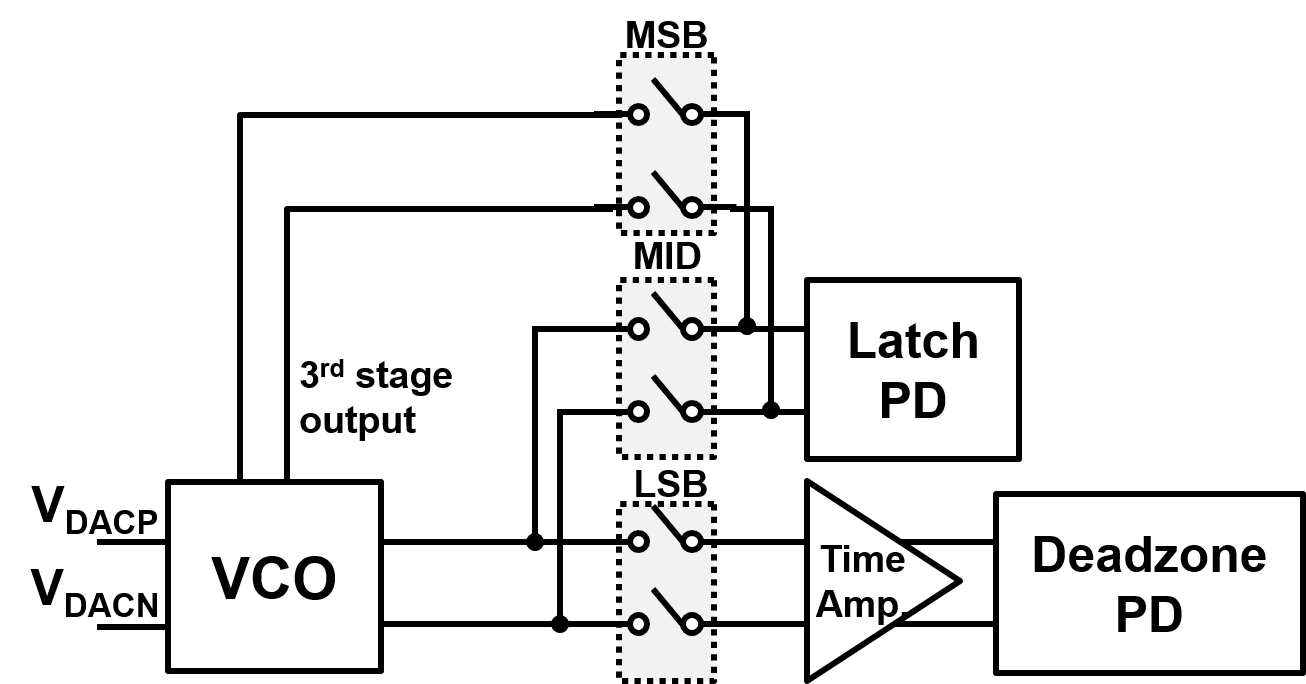
\includegraphics[width=0.5\textwidth]{figs/vco-entire.png}
\caption{The complete VCO-based comparator schematic. The comparator switches to 3 noise mode depending on the SA cycle with simple CMOS switches.}
\label{fullvco}
\end{figure}

High-precision SAR ADCs are often designed with redundancy to mitigate the effects of C-DAC and reference settling. Since the comparator noise requirements differ according to the SA cycles, it is useful if the comparator noise mode can be digitally configured.
Our 13-bit SAR ADC holds 2-bit redundancy: since redundancy is assigned to each bit, even if a judgment error occurs in the upper MSB bits, errors can be corrected with fine bit decisions in the LSB comparisons\cite{kapusta201314b}. For example, the upper 5 bits can tolerate a decision error equivalent to 200 LSBs. It would be a waste of energy to use a VCO-based comparator with LSB-level accuracy in the MSBs.

As in Fig.\ref{fullvco}, we propose a VCO-based comparator with digitally configurable noise performance. 
The main idea is to use a delay line-based comparator with a feed-forward latch to minimize power consumption during MSB comparisons, where accuracy is not required. During LSB comparisons, we switch to a VCO-based comparator with deadzone PDs. A simple switching circuit allows the VCO-based comparator with three noise modes, and the specific implementation is as follows:
\begin{itemize}
\item \textbf{MSB mode} (first 5 SA cycles): Operates as a simple 3-stage delay line, since it can tolerate large judgment errors. IRN:2mVpp.
\item \textbf{MID mode} (middle 5 SA cycles): Operates as an 11-stage delay line. IRN:240uVpp.
\item \textbf{LSB mode} (last 5 SA cycles): 11-stage VCO operation as described in Chapter 3. IRN:75uVpp.
\end{itemize}
In the MSB and MID modes, latch-based PD is used to force decisions with positive feedback. Such PDs are noisier, but do not have deadzones, and are power-efficient.
In our implementation, since multiple latches are used, different offsets will be generated depending on the cycle. These offsets are absorbed by the redundancy of the SAR ADC, and the mismatch-related latch offsets are designed to be within the redundancy range.

\subsection{VCO and Time Amp. designs}
\begin{figure}[!]
\centering
 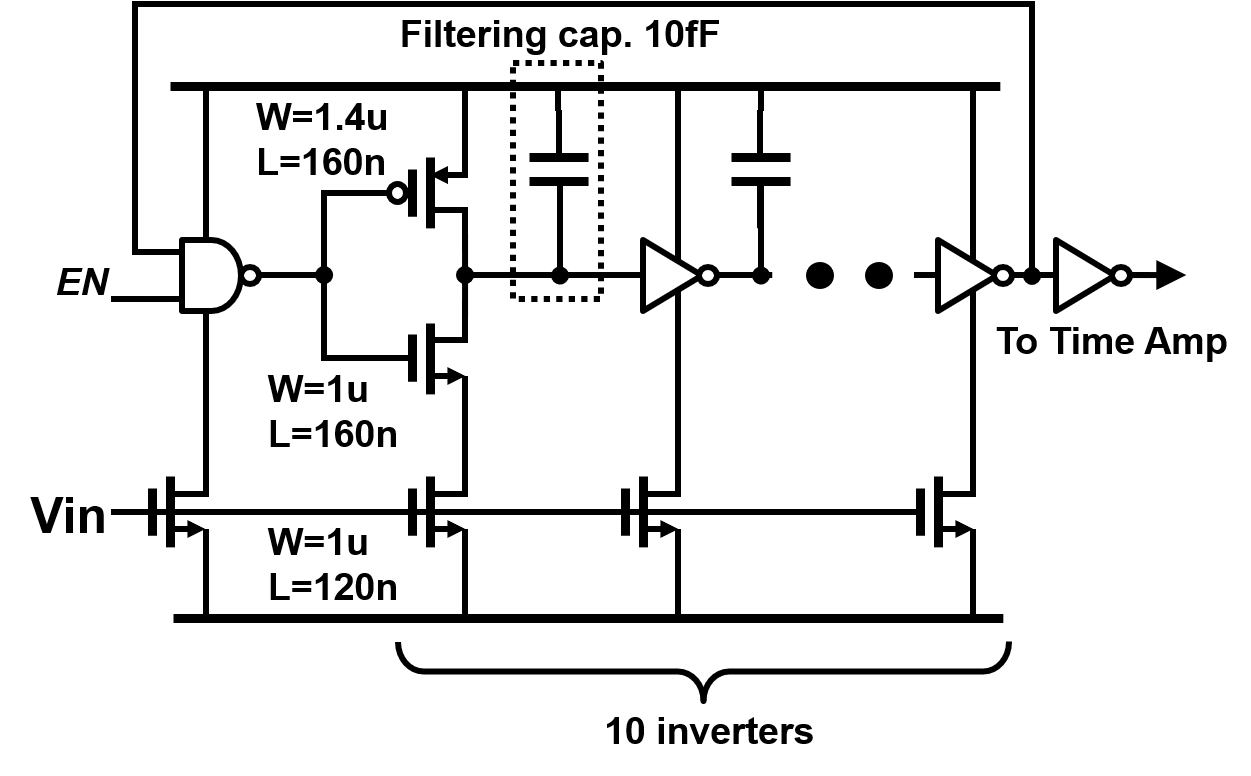
\includegraphics[width=0.5\textwidth]{figs/vco_cell.png}
  \caption{Ring-VCO transistor schematic.}
  \label{cell}
\end{figure}

\begin{figure}[!]
\centering
 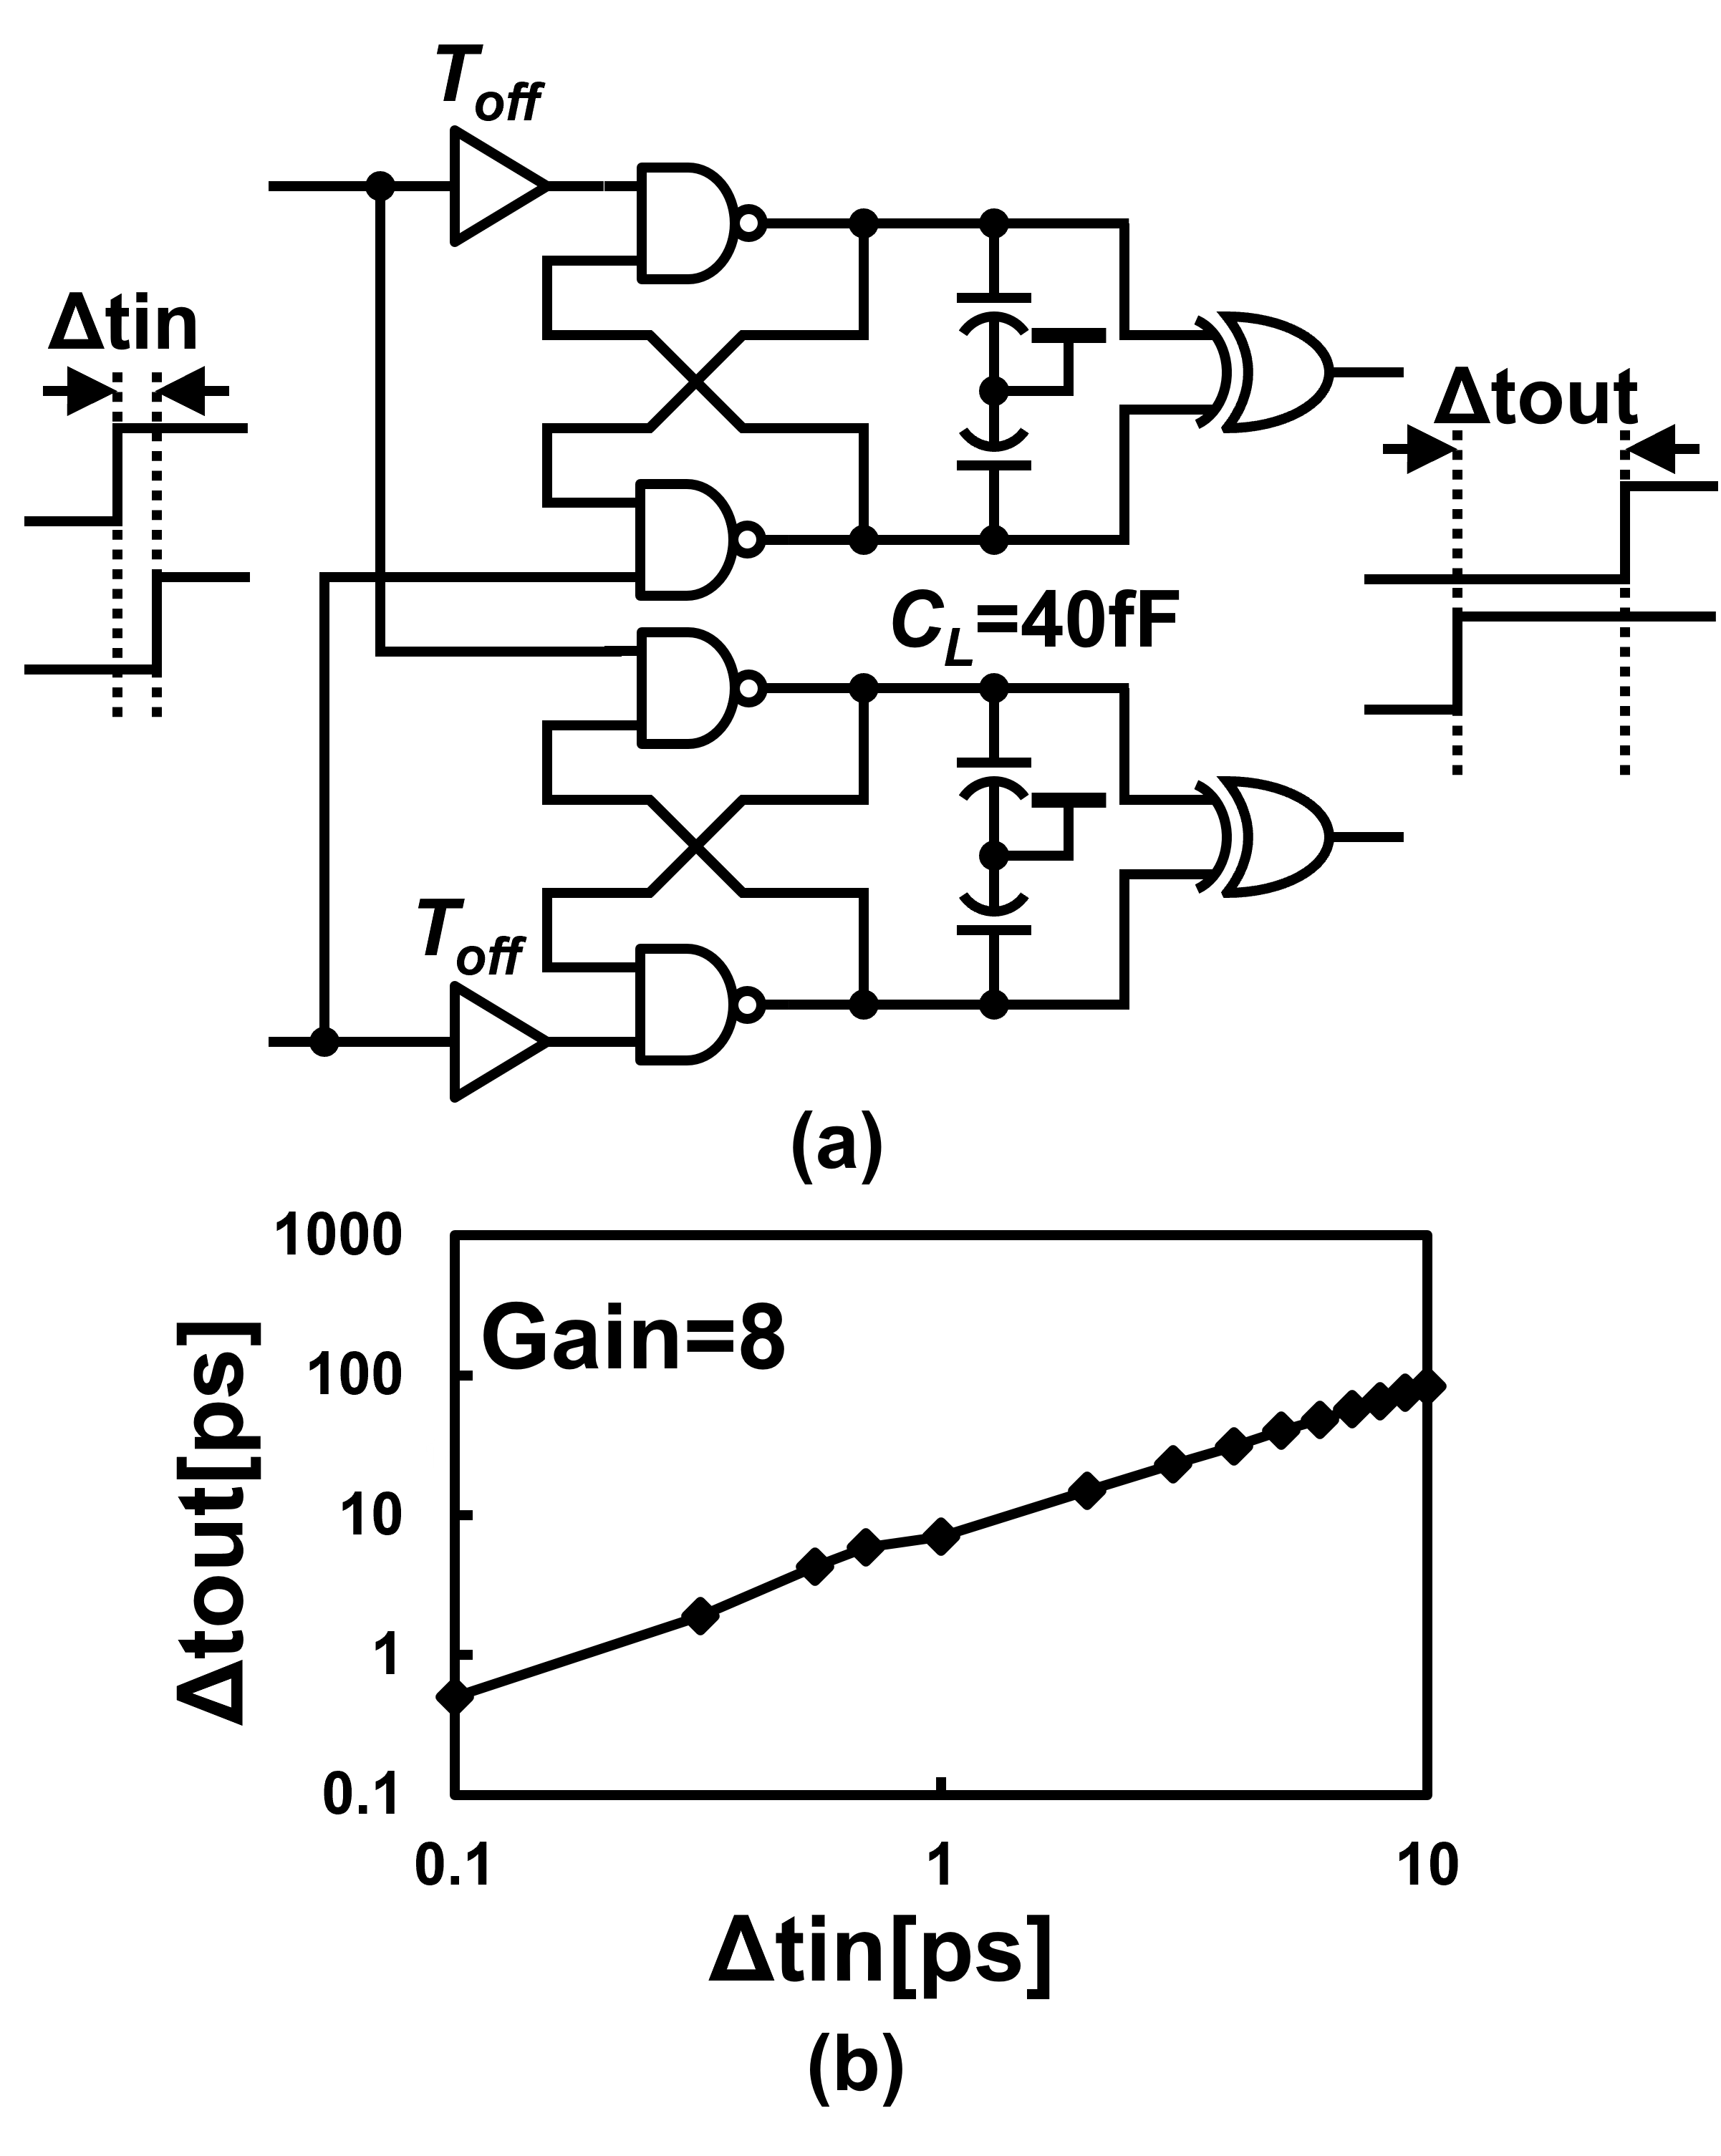
\includegraphics[width=0.5\textwidth]{figs/ta_chara.png}
  \caption{(a) Time amplifier schematic based on ref.\cite{timecomp}. (b) Simulated amplification characteristics.}
  \label{timeamp}
\end{figure}

\textcolor{red}{Finally, we describe the design of the VCO cell and time amplifier. As shown in Fig.\ref{cell}, the VCO cell achieves voltage-time conversion by binding the NMOS side of the inverter in a current-starving fashion. 
There is an important power-speed tradeoff in the design of VCO comparators. The PMOS side can also be current-starved to increase the VCO voltage-time conversion gain\cite{shim2017edge}\cite{timecomp}, which will significantly improve the comparator noise performance and ADC power efficiency. However, when the PMOS is also tied, the VCO oscillation frequency drops significantly. In our design, the NMOS+PMOS tied VCO failed to meet our target of 1MS/s SAR ADC operation and such design choice was not taken.}

The VCO in this design is designed to oscillate at 600MHz with $V_{DD}$=1.2V and a common-mode voltage of 500mV is given, which is a sufficient speed for 1MS/s SAR ADCs. While the tail NMOS $g_m$ should be maximized to suppress noise, the gate leakage currents contributed to the accuracy degradation in our design. Thus, the L sizing was increased to mitigate this effect. 

Our time amplifier is designed based on ref.\cite{lee20089}, and the schematics and simulated amplification characteristics are shown in Fig.\ref{timeamp}. 
\textcolor{red}{Although nonlinearity is noticeable, it does not affect the accuracy of the comparator as long as the monotonicity is maintained.}
Following ref.\cite{lee20089}, $G_{TA}$ is given by:
\begin{eqnarray}
    \centering
    G_{TA} = \frac{2C_L}{g_mT_{off}}
    \label{gta}
\end{eqnarray}
As mentioned in the previous section, under FF high-temperature conditions $G_{TA}$ drops, since the gain is inversely proportional to $g_m$.
In this design, the gain at TT condition is designed to be 8 by tuning $T_{off}$ and the load capacitance. Moreover, while not implemented in this design, $G_{TA}$ can be easily configured by digitally switching $C_L$. By such mechanisms, we can digitally control the noise performance of the VCO-based comparator and such configuration can become useful when designing ADCs for multiple resolution modes\cite{harpe201310b}.

% ここまで書いた
\section{Experiment Results}
\begin{figure}[!t]
\centering
 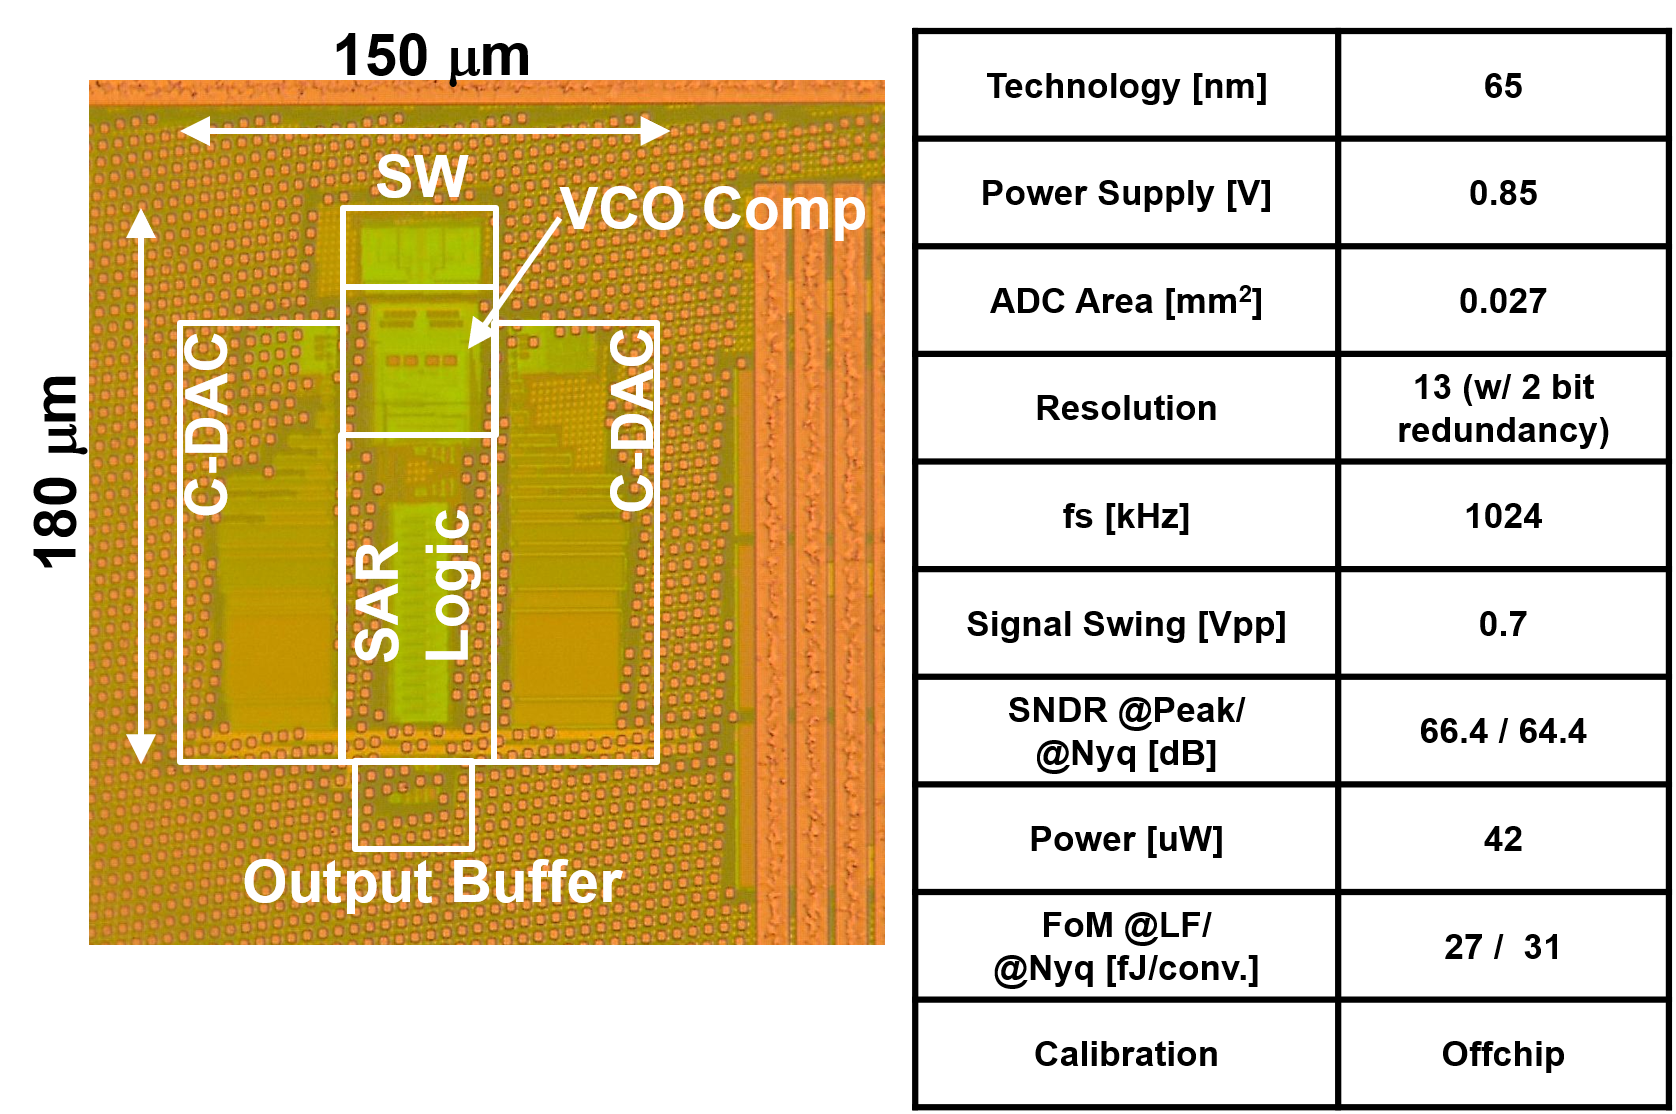
\includegraphics[width=0.5\textwidth]{figs/chipphoto.png}
  \caption{Chip micrograph and performance summary of the ADC.}
  \label{chipphoto}
\end{figure}

\begin{figure}[!t]
\centering
 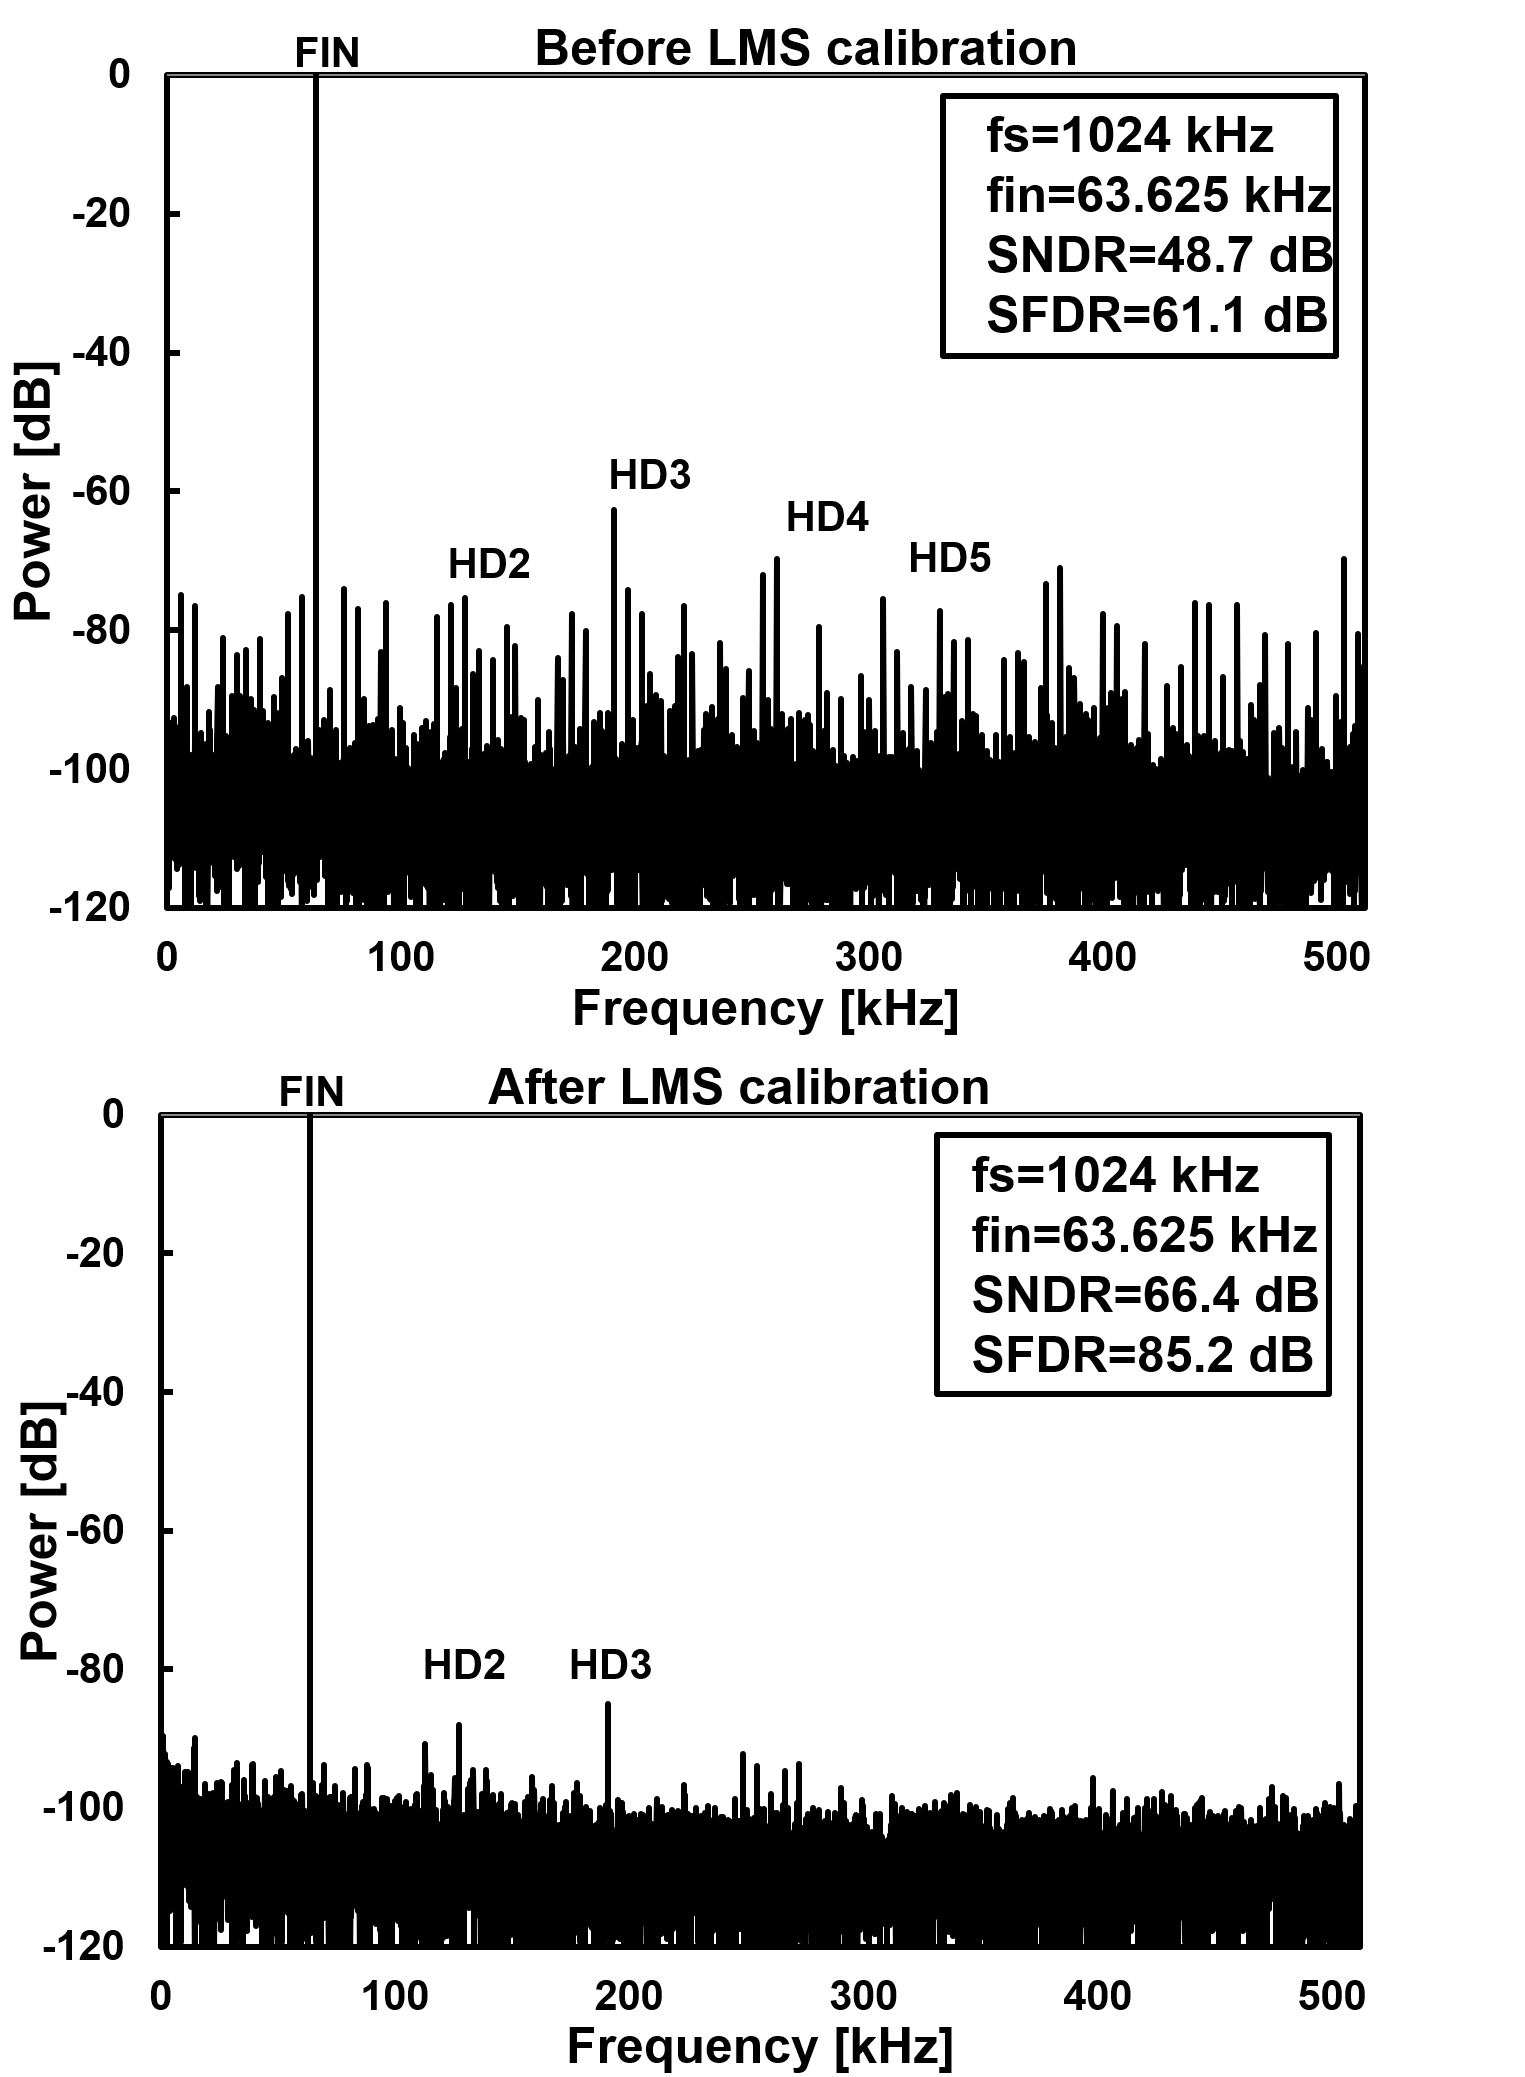
\includegraphics[width=0.5\textwidth]{figs/fft.png}
  \caption{16384 FFT results before and after LMS calibration.}
  \label{aftercal}
\end{figure}

\begin{figure}[!t]
\centering
 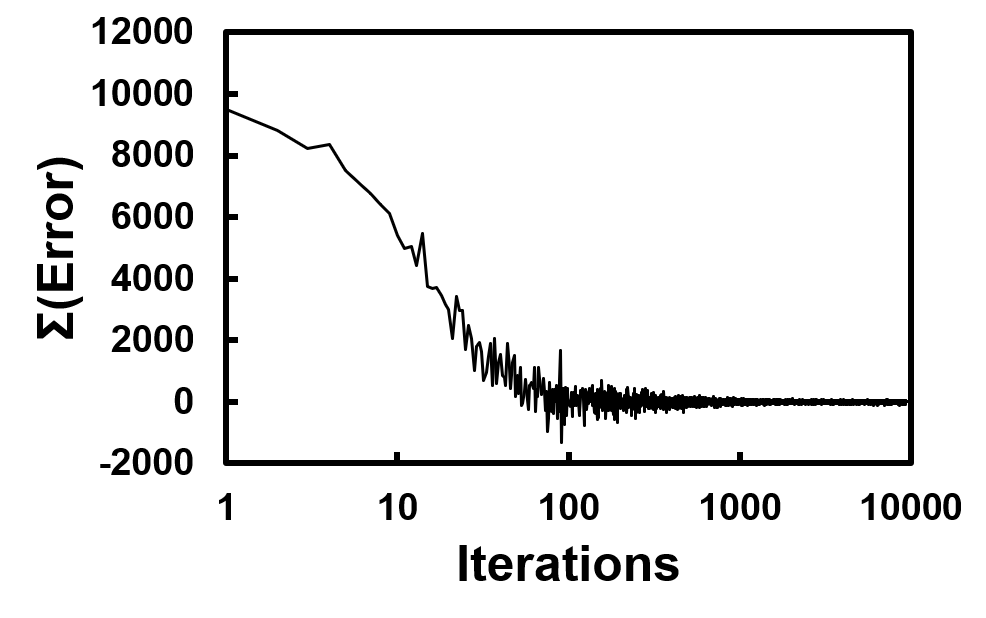
\includegraphics[width=0.45\textwidth]{figs/lms.png}
  \caption{LMS calibration error convergence. With sufficient hyper-parameter settings, the C-DAC linearity reaches 12-bit level by 5000 iterations. }
  \label{lms}
\end{figure}

\begin{figure}[!t]
\centering
 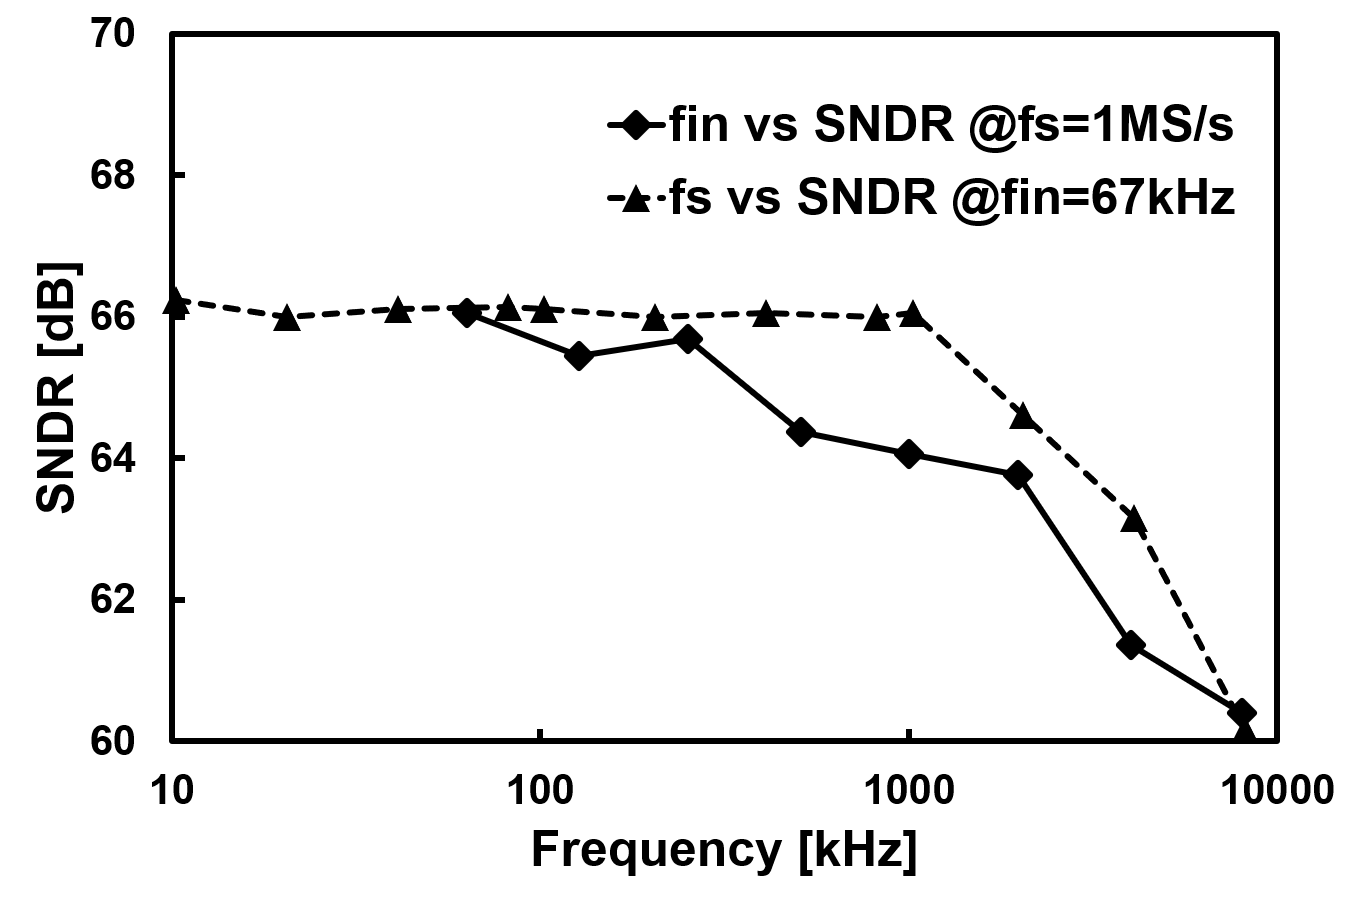
\includegraphics[width=0.5\textwidth]{figs/freq-sndr.png}
  \caption{Measured fin and fs versus SNDR characteristics, respectively.}
  \label{freqvssndr}
\end{figure}

\begin{figure}[!t]
\centering
 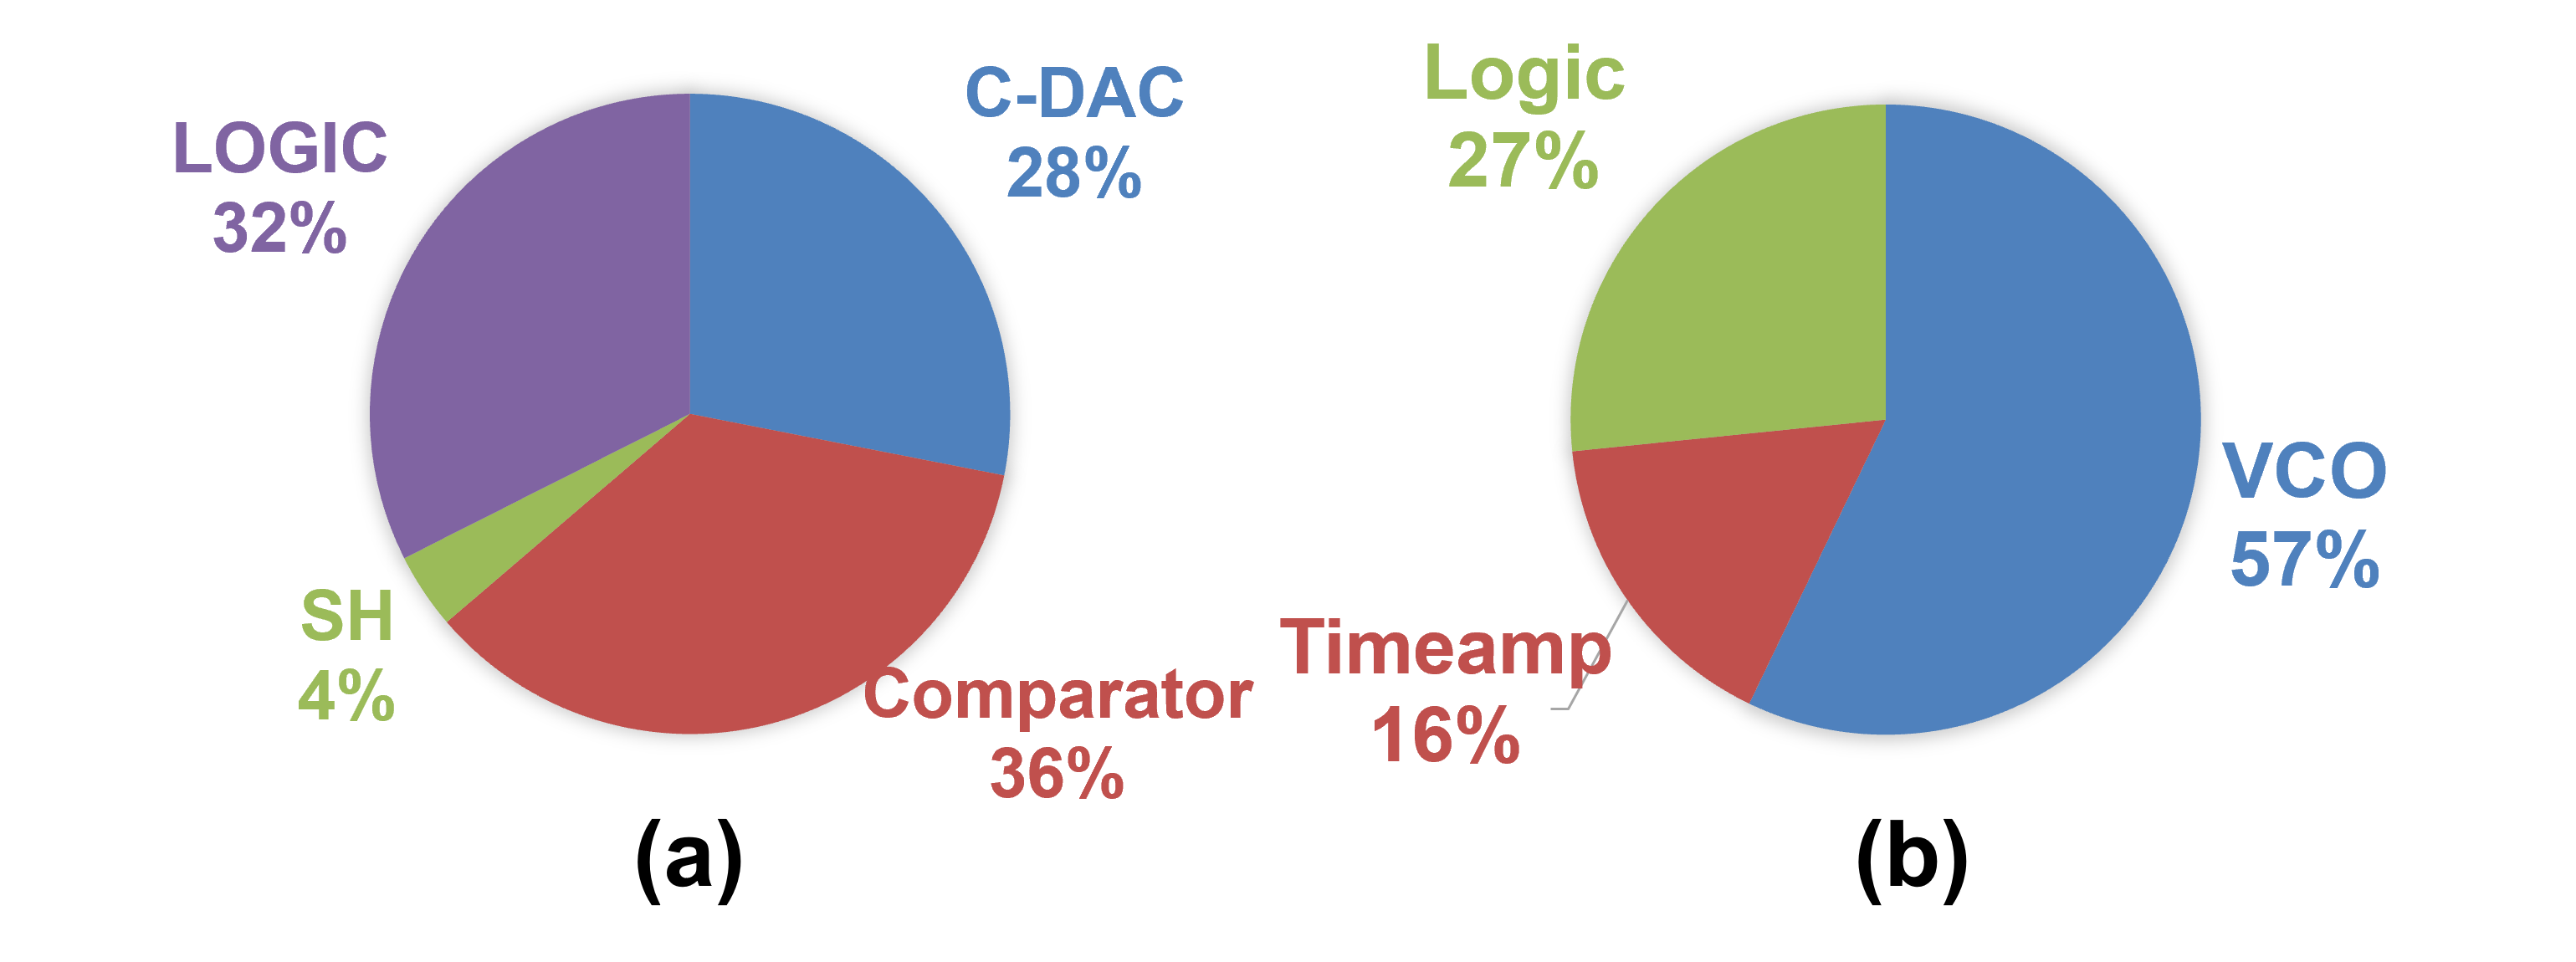
\includegraphics[width=0.52\textwidth]{figs/breakdown.png}
 \caption{\textcolor{red}{(a) Simulated power breakdown of the ADC. (b) Simulated power breakdown of the VCO comparator}}
  \label{power}
\end{figure}

The SAR ADC was fabricated in 65-nm CMOS and Fig.\ref{chipphoto} shows the chip micrograph and a performance summary. 
Fig.\ref{aftercal} shows the result of 16384-FFT before and after LMS calibration. The two FFT results were lead using the same raw data, but different bit weighting was used: the prior uses the weighting as in the schematic, and the latter uses weighting derived via LMS calibration. Therefore, the noise situation is the same. Even though we do not add any tuning to the VCO-based comparator in this design, fine noise performance was achieved. 

Fig.\ref{lms} shows the LMS calibration iteration versus the error convergence. With sufficient hyper-parameters, the LMS engine requires about 5000 iterations for convergence. After the convergence, the perturbation injection can be stopped to save power. 
We would like to note that the power consumption shown in Fig.\ref{chipphoto} is measured when the perturbation injection is turned off. If the LMS calibration engine was to be implemented on-chip and run background, we expect that the total ADC power consumption will increase 3x. 

We plot fs and fin versus SNDR respectively in Fig.\ref{freqvssndr}. Since the VCO-based comparator is mostly digital, low voltage operation was easily accomplished. All of the measurements have been carried out with a single supply voltage of 0.85V. At 1.2V supply, the ADC achieves similar SNDR performance and extends fs to 10MS/s, but with a worsened power efficiency. In addition, we must be careful of the signal common-mode voltage ($V_{CM}$) since this directly impacts the inverter’s $I_{DS}$ in eq.(\ref{delaylineIRN}). When the $V_{CM}$ was increased beyond 0.5V, degradation in SNDR was observed.

\begin{table*}[!]
\centering
 \caption{\textcolor{red}{Performance comparison between low-power SAR ADCs.}}
 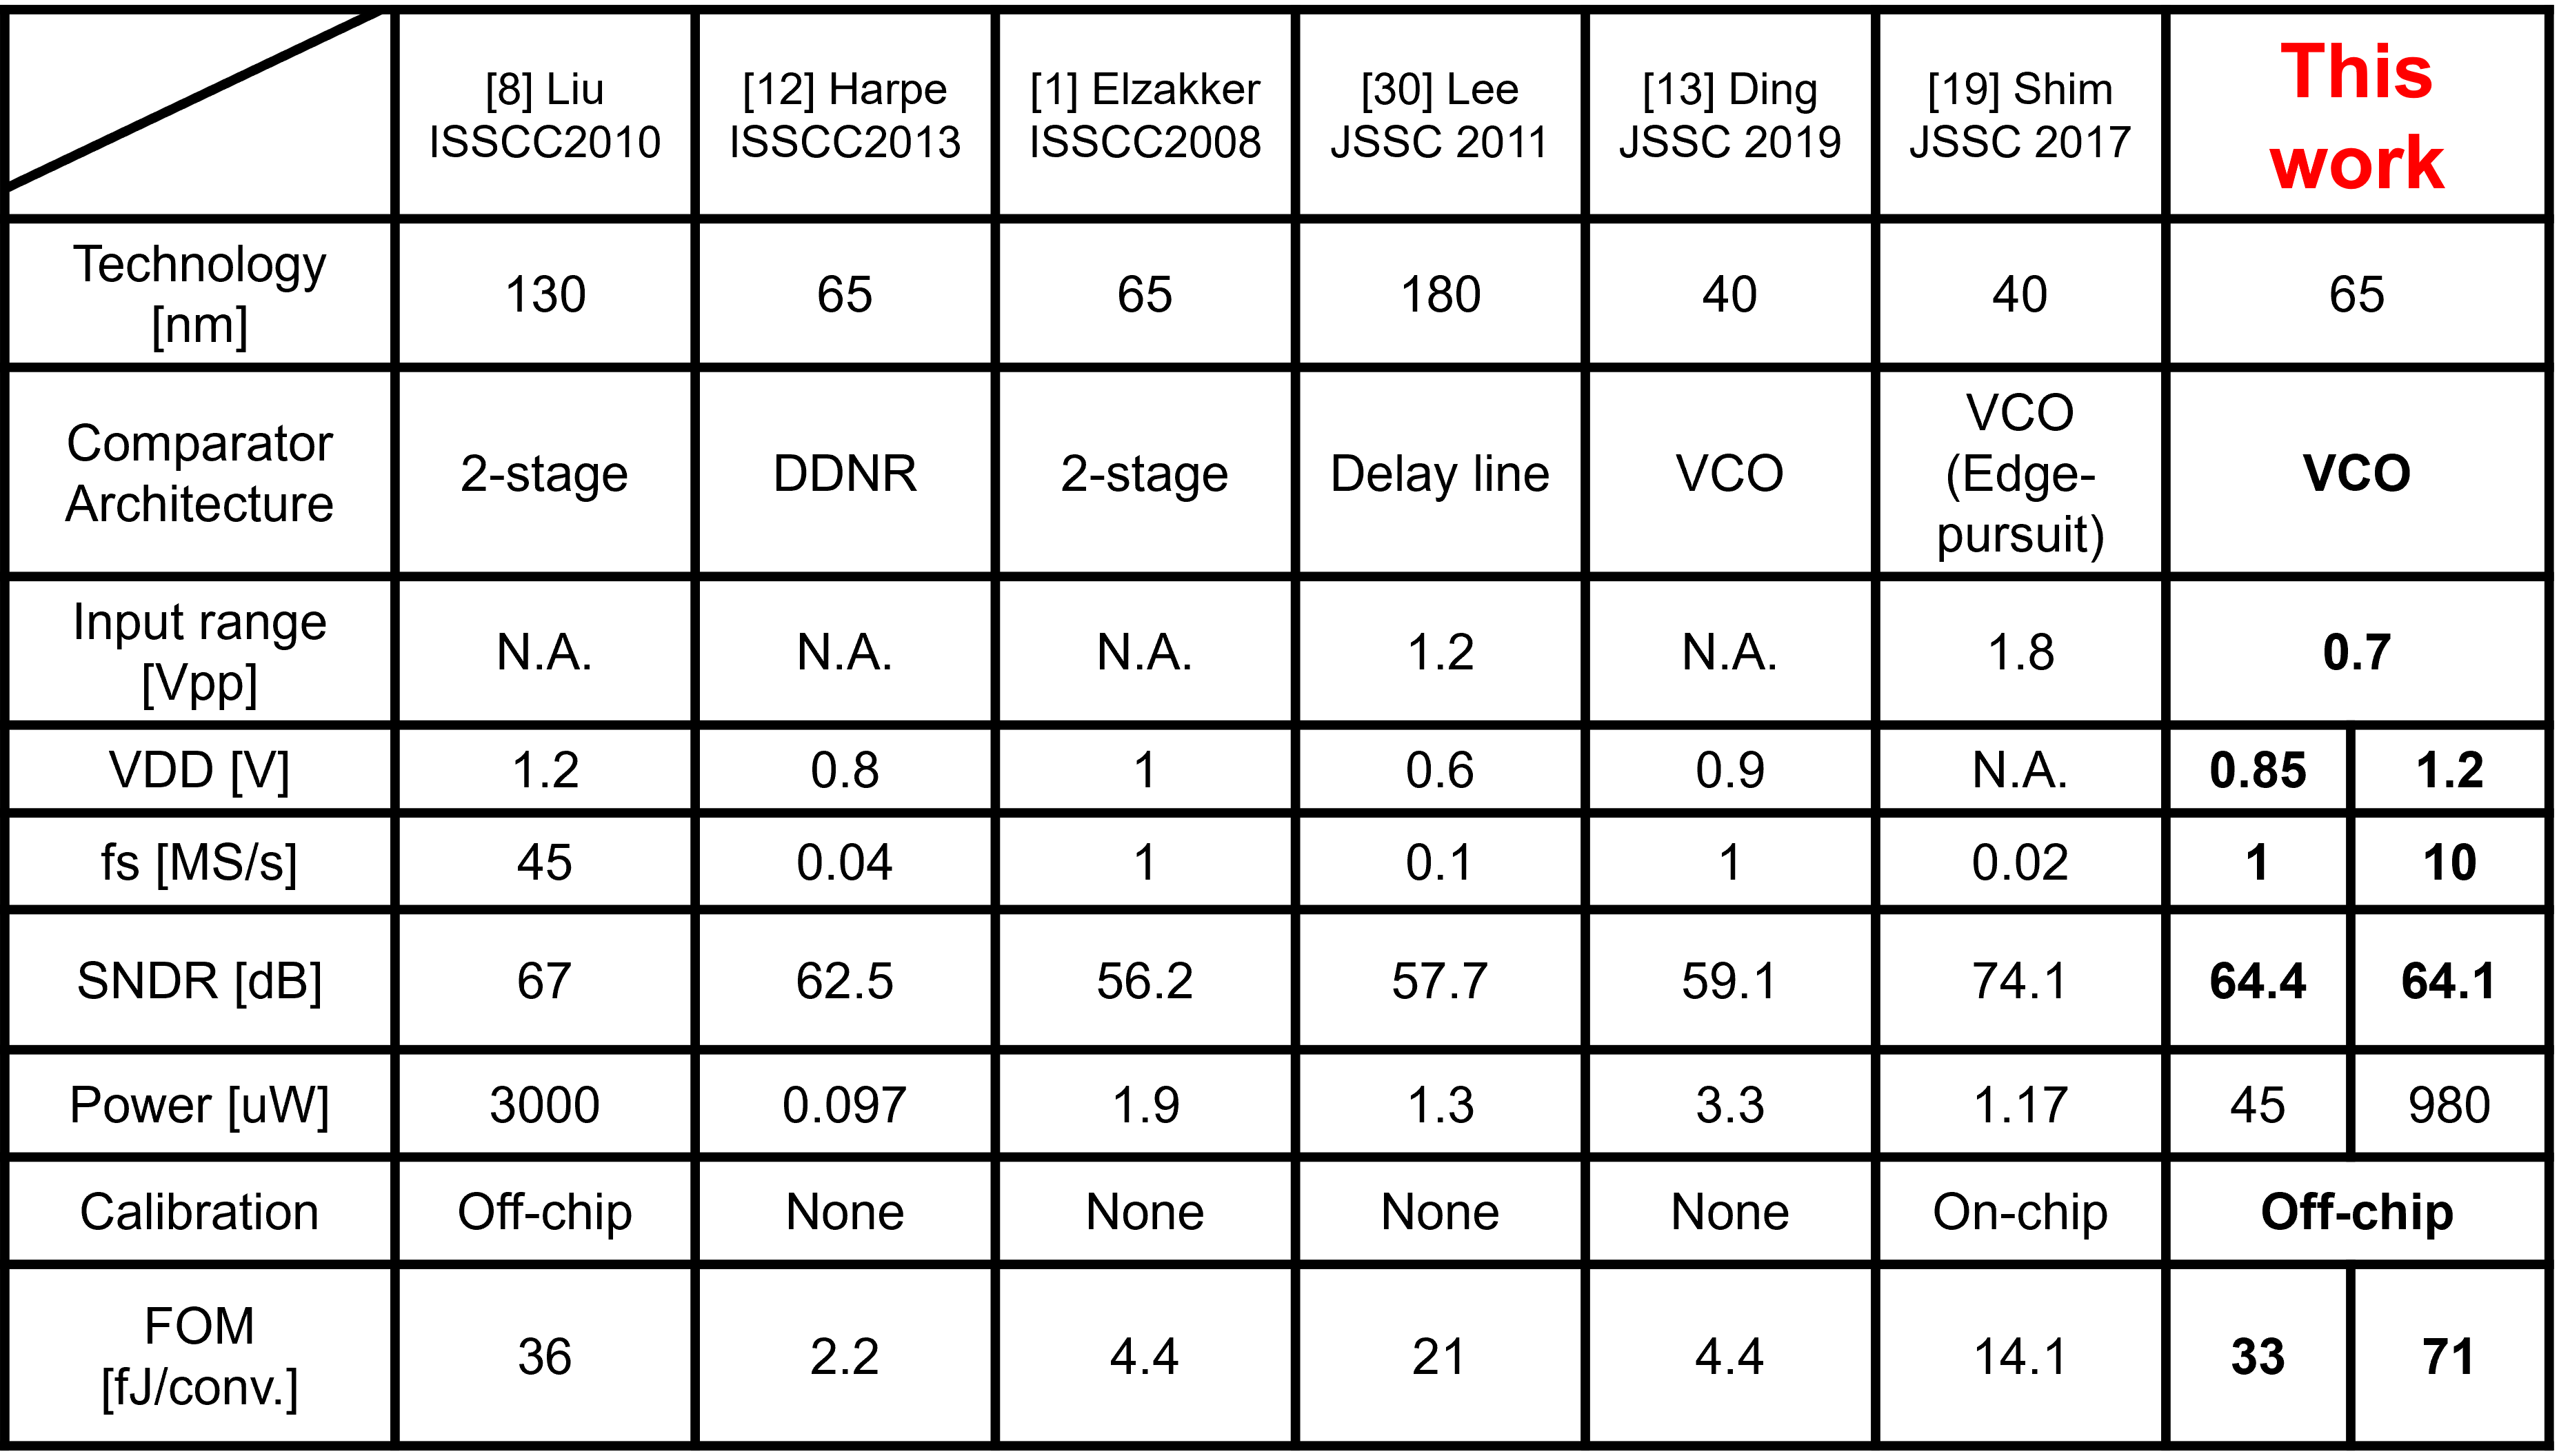
\includegraphics[width=0.9\textwidth]{figs/table.png}
  \label{performancecomp}
\end{table*}

Finally, we conduct a performance comparison with low-power SAR ADCs in Table \ref{performancecomp}. Our SAR ADC is the first to achieve fully adaptive noise scaling for high-resolution comparators, which opens a new field of research upon further power reduction of the comparator power consumption. 

\textcolor{red}{Innovative VCO comparator designs like edge-pursuit comparator (EPC) \cite{shim2017edge} achieves both higher SNDR and power efficiencies than our design. EPC requires only a single VCO for the comparison and is low-power. However, the VCO must tie both NMOS and PMOS and the VCO oscillation frequency is degraded and the SAR ADC speed is slow (20kS/s).}

\textcolor{red}{Fig.\ref{power}(a) shows the power breakdown of the ADC, where the VCO comparator is 36\% of the ADC power, balanced with other blocks. A detailed power breakdown of the VCO comparator is also added in Fig.\ref{power}(b) for further reference: the VCO itself dominates with 57\% of the power, while logic power such as time amp and phase detector is small.}

One of the reasons of the worsened FoM (peak of 29fJ/conv.) were the limitations in the measurement environment. Due to the poor IP3 performance of the signal generator, the signal input swing was limited to $0.7V_{pp}$, which occupied only half of the SAR ADC input range. The SNDR was limited to 66.4 dB, but achieving full-scale input should further extend the SNDR around 3-4dB without power overheads. 

\section{Conclusions}
To realize a fully adaptive noise scaling comparator, a VCO-based comparator with an eye-opening technique was introduced.  Even though the proposed VCO-based comparator was designed for a 13-bit ADC, this comparator can be extended further resolutions by carefully designing the jitter performance and the deadzone, as analyzed in this paper. Moreover, since the VCO-based comparator is mainly based on inverters and other simple logic cells, the comparator receives full benefits from process scaling. %Furthermore, the comparator characteristics can be analyzed with well-known knowledge of ring-oscillators. 

\bibliographystyle{IEEEbib}
\bibliography{main}


\begin{IEEEbiography}
[{
\includegraphics[width=1in,height=1.25in,clip,keepaspectratio]{bio/1.jpg}}]{Kentaro Yoshioka}
received his BS, MS, Ph.D degrees from Keio University, Japan. Currently, he is an Assistant Professor at Keio University. He worked with Toshiba during 2014-2021, developing circuitry for WiFi and LiDAR SoCs. During 2017-2018, he had been a visiting scholar at Stanford University, exploring efficient machine learning hardware and algorithms. 

Currently, Dr. Yoshioka serves as a technical program member of Symp. VLSI circuits conference. He was the recipient of ASP-DAC 2013 Special Feature Award, the A-SSCC 2012 Best Design Award, and 1st place winner of Kaggle 2020 Prostate Cancer Grade Assessment (PANDA) Challenge.
\end{IEEEbiography}

\end{document}
